% Options for packages loaded elsewhere
\PassOptionsToPackage{unicode}{hyperref}
\PassOptionsToPackage{hyphens}{url}
%
\documentclass[
]{book}
\usepackage{amsmath,amssymb}
\usepackage{lmodern}
\usepackage{ifxetex,ifluatex}
\ifnum 0\ifxetex 1\fi\ifluatex 1\fi=0 % if pdftex
  \usepackage[T1]{fontenc}
  \usepackage[utf8]{inputenc}
  \usepackage{textcomp} % provide euro and other symbols
\else % if luatex or xetex
  \usepackage{unicode-math}
  \defaultfontfeatures{Scale=MatchLowercase}
  \defaultfontfeatures[\rmfamily]{Ligatures=TeX,Scale=1}
\fi
% Use upquote if available, for straight quotes in verbatim environments
\IfFileExists{upquote.sty}{\usepackage{upquote}}{}
\IfFileExists{microtype.sty}{% use microtype if available
  \usepackage[]{microtype}
  \UseMicrotypeSet[protrusion]{basicmath} % disable protrusion for tt fonts
}{}
\makeatletter
\@ifundefined{KOMAClassName}{% if non-KOMA class
  \IfFileExists{parskip.sty}{%
    \usepackage{parskip}
  }{% else
    \setlength{\parindent}{0pt}
    \setlength{\parskip}{6pt plus 2pt minus 1pt}}
}{% if KOMA class
  \KOMAoptions{parskip=half}}
\makeatother
\usepackage{xcolor}
\IfFileExists{xurl.sty}{\usepackage{xurl}}{} % add URL line breaks if available
\IfFileExists{bookmark.sty}{\usepackage{bookmark}}{\usepackage{hyperref}}
\hypersetup{
  pdftitle={Boosting methods: Theory and application in R},
  pdfauthor={Emanuel Sommer},
  hidelinks,
  pdfcreator={LaTeX via pandoc}}
\urlstyle{same} % disable monospaced font for URLs
\usepackage{color}
\usepackage{fancyvrb}
\newcommand{\VerbBar}{|}
\newcommand{\VERB}{\Verb[commandchars=\\\{\}]}
\DefineVerbatimEnvironment{Highlighting}{Verbatim}{commandchars=\\\{\}}
% Add ',fontsize=\small' for more characters per line
\usepackage{framed}
\definecolor{shadecolor}{RGB}{248,248,248}
\newenvironment{Shaded}{\begin{snugshade}}{\end{snugshade}}
\newcommand{\AlertTok}[1]{\textcolor[rgb]{0.94,0.16,0.16}{#1}}
\newcommand{\AnnotationTok}[1]{\textcolor[rgb]{0.56,0.35,0.01}{\textbf{\textit{#1}}}}
\newcommand{\AttributeTok}[1]{\textcolor[rgb]{0.77,0.63,0.00}{#1}}
\newcommand{\BaseNTok}[1]{\textcolor[rgb]{0.00,0.00,0.81}{#1}}
\newcommand{\BuiltInTok}[1]{#1}
\newcommand{\CharTok}[1]{\textcolor[rgb]{0.31,0.60,0.02}{#1}}
\newcommand{\CommentTok}[1]{\textcolor[rgb]{0.56,0.35,0.01}{\textit{#1}}}
\newcommand{\CommentVarTok}[1]{\textcolor[rgb]{0.56,0.35,0.01}{\textbf{\textit{#1}}}}
\newcommand{\ConstantTok}[1]{\textcolor[rgb]{0.00,0.00,0.00}{#1}}
\newcommand{\ControlFlowTok}[1]{\textcolor[rgb]{0.13,0.29,0.53}{\textbf{#1}}}
\newcommand{\DataTypeTok}[1]{\textcolor[rgb]{0.13,0.29,0.53}{#1}}
\newcommand{\DecValTok}[1]{\textcolor[rgb]{0.00,0.00,0.81}{#1}}
\newcommand{\DocumentationTok}[1]{\textcolor[rgb]{0.56,0.35,0.01}{\textbf{\textit{#1}}}}
\newcommand{\ErrorTok}[1]{\textcolor[rgb]{0.64,0.00,0.00}{\textbf{#1}}}
\newcommand{\ExtensionTok}[1]{#1}
\newcommand{\FloatTok}[1]{\textcolor[rgb]{0.00,0.00,0.81}{#1}}
\newcommand{\FunctionTok}[1]{\textcolor[rgb]{0.00,0.00,0.00}{#1}}
\newcommand{\ImportTok}[1]{#1}
\newcommand{\InformationTok}[1]{\textcolor[rgb]{0.56,0.35,0.01}{\textbf{\textit{#1}}}}
\newcommand{\KeywordTok}[1]{\textcolor[rgb]{0.13,0.29,0.53}{\textbf{#1}}}
\newcommand{\NormalTok}[1]{#1}
\newcommand{\OperatorTok}[1]{\textcolor[rgb]{0.81,0.36,0.00}{\textbf{#1}}}
\newcommand{\OtherTok}[1]{\textcolor[rgb]{0.56,0.35,0.01}{#1}}
\newcommand{\PreprocessorTok}[1]{\textcolor[rgb]{0.56,0.35,0.01}{\textit{#1}}}
\newcommand{\RegionMarkerTok}[1]{#1}
\newcommand{\SpecialCharTok}[1]{\textcolor[rgb]{0.00,0.00,0.00}{#1}}
\newcommand{\SpecialStringTok}[1]{\textcolor[rgb]{0.31,0.60,0.02}{#1}}
\newcommand{\StringTok}[1]{\textcolor[rgb]{0.31,0.60,0.02}{#1}}
\newcommand{\VariableTok}[1]{\textcolor[rgb]{0.00,0.00,0.00}{#1}}
\newcommand{\VerbatimStringTok}[1]{\textcolor[rgb]{0.31,0.60,0.02}{#1}}
\newcommand{\WarningTok}[1]{\textcolor[rgb]{0.56,0.35,0.01}{\textbf{\textit{#1}}}}
\usepackage{longtable,booktabs,array}
\usepackage{calc} % for calculating minipage widths
% Correct order of tables after \paragraph or \subparagraph
\usepackage{etoolbox}
\makeatletter
\patchcmd\longtable{\par}{\if@noskipsec\mbox{}\fi\par}{}{}
\makeatother
% Allow footnotes in longtable head/foot
\IfFileExists{footnotehyper.sty}{\usepackage{footnotehyper}}{\usepackage{footnote}}
\makesavenoteenv{longtable}
\usepackage{graphicx}
\makeatletter
\def\maxwidth{\ifdim\Gin@nat@width>\linewidth\linewidth\else\Gin@nat@width\fi}
\def\maxheight{\ifdim\Gin@nat@height>\textheight\textheight\else\Gin@nat@height\fi}
\makeatother
% Scale images if necessary, so that they will not overflow the page
% margins by default, and it is still possible to overwrite the defaults
% using explicit options in \includegraphics[width, height, ...]{}
\setkeys{Gin}{width=\maxwidth,height=\maxheight,keepaspectratio}
% Set default figure placement to htbp
\makeatletter
\def\fps@figure{htbp}
\makeatother
\setlength{\emergencystretch}{3em} % prevent overfull lines
\providecommand{\tightlist}{%
  \setlength{\itemsep}{0pt}\setlength{\parskip}{0pt}}
\setcounter{secnumdepth}{5}
\usepackage{booktabs}
\usepackage{array}
\ifluatex
  \usepackage{selnolig}  % disable illegal ligatures
\fi
\usepackage[]{natbib}
\bibliographystyle{apalike}
\newlength{\cslhangindent}
\setlength{\cslhangindent}{1.5em}
\newlength{\csllabelwidth}
\setlength{\csllabelwidth}{3em}
\newenvironment{CSLReferences}[2] % #1 hanging-ident, #2 entry spacing
 {% don't indent paragraphs
  \setlength{\parindent}{0pt}
  % turn on hanging indent if param 1 is 1
  \ifodd #1 \everypar{\setlength{\hangindent}{\cslhangindent}}\ignorespaces\fi
  % set entry spacing
  \ifnum #2 > 0
  \setlength{\parskip}{#2\baselineskip}
  \fi
 }%
 {}
\usepackage{calc}
\newcommand{\CSLBlock}[1]{#1\hfill\break}
\newcommand{\CSLLeftMargin}[1]{\parbox[t]{\csllabelwidth}{#1}}
\newcommand{\CSLRightInline}[1]{\parbox[t]{\linewidth - \csllabelwidth}{#1}\break}
\newcommand{\CSLIndent}[1]{\hspace{\cslhangindent}#1}

\title{Boosting methods: Theory and application in R}
\author{Emanuel Sommer}
\date{2021-04-30}

\begin{document}
\maketitle

{
\setcounter{tocdepth}{1}
\tableofcontents
}
\hypertarget{prerequisites}{%
\chapter{Prerequisites}\label{prerequisites}}

The reader should have some basic knowledge of the following topics:

\begin{itemize}
\item
  Statistical learning

  \begin{itemize}
  \item
    Train/ test split
  \item
    Cross-validation
  \item
    Overfitting
  \item
    Gradient descent
  \item
    Bias variance trade-off
  \item
    Hyperparameters
  \end{itemize}
\item
  Regression trees and random forest models
\item
  Basic R knowledge (only for the applied part)
\end{itemize}

\hypertarget{intro}{%
\chapter{Introduction}\label{intro}}

This bookdown project shows my work for the main master's seminar from my \emph{M.Sc. Mathematics in Data Science} at the TUM. The topic of the seminar is \emph{Statistical Methods and Models}. During the seminar I was supervised by Prof.~Claudia Czado and Özge Sahin. My topic and thus covered in this project are boosting methods. Those are unarguably one of the hottest machine learning algorithms for tabular data to date.

\begin{quote}
``Boosting is one of the most powerful learning ideas introduced in the last
twenty years.'' \citep{elements}
\end{quote}

Hereby the focus will lie on the regression and not the more often discussed classification setting. The main idea of boosting is to sequentially build models from some class of base learners to finally combine them to a powerful ensemble model. As the base learners regression trees will be chosen in this project.

The next chapter will cover the theory behind boosting and especially tree-based gradient boosting. Besides a very prominent, efficient and successful implementation of tree-based gradient boosting namely XGBoost will be discussed in this chapter. It gained a lot of attention when it was integral to many winning submissions in machine learning competitions on the platform Kaggle and comes with some interesting tweaks to the general algorithm.

The application of the discussed boosting models to two real world data sets with the use of the programming language R are the content of the subsequent chapters. This will be divided into exploratory data analysis and the modeling itself. Notably the framework of \texttt{tidymodels} is used in the practical part.

\hypertarget{theory}{%
\chapter{Theory}\label{theory}}

\hypertarget{the-powerful-idea-of-gradient-boosting}{%
\section{The powerful idea of gradient boosting}\label{the-powerful-idea-of-gradient-boosting}}

As roughly mentioned in the introduction section \ref{intro} the main idea of boosting is to sequentially build weak learners that form a powerful ensemble model. With weak learners models with high bias and low variance are meant that perform at least a little better than guessing. This already shows that the sequential approach of gradient boosting with `weak' learners stands in strong contrast to bagged ensembles like random forest. There many models with low bias and high variance are fitted in a parallel fashion and the variance is then reduced by averaging over the models.\citep{HandsOnMLwithR} It is not totally clear from which field boosting methods emerged but some claim that the work of Freund and Schapire with respect to PAC learning in the 1990s were instrumental for their growth.\citep{elements} PAC learning can be considered one field within the broader field of learning theory that tries to find generalization bounds for algorithms that are probably approximately correct (PAC).\citep{pacbounds} This section will first cover the general setup of gradient boosting as the most prominent method to train forward stagewise additive models. Secondly tree-based gradient boosting and finally a very efficient and robust tree-based gradient boosting algorithm namely XGBoost will be discussed in detail.

\hypertarget{forward-stagewise-additive-modeling}{%
\subsection{Forward Stagewise Additive Modeling}\label{forward-stagewise-additive-modeling}}

In the setting of the dataset \(\mathcal{D} = \{(y_i,x_i)\ | i \in [N]\}\) with predictors \(x_i \in \mathbb{R}^m\) and target \(y_i \in \mathbb{R}\) boosting is fitting the following additive, still quite general, model.

\begin{equation}
  \hat{y_i} = \phi(x_i) = \sum_{k=1}^{K} f_k(x_i), \quad f_k \in \mathcal{F}
  \label{eq:additiveModel}
\end{equation}

Where \(\mathcal{F}\) is the space of learning algorithms that will be narrowed down later on. Additive expansions like this are at the core of many other powerful machine learning algorithms like Neural Networks or Wavelets.\citep{elements}

The formulation \eqref{eq:additiveModel} leads to so called forward stagewise additive modeling which basically means that one sequentially adds \(f \in \mathcal{F}\) to the current model \(\phi_k\) without changing anything about the previous models.\citep{elements} The algorithm is shown below.

\begin{center}\rule{0.5\linewidth}{0.5pt}\end{center}

\textbf{Algorithm 1}: Forward Stagewise Additive Modeling \citep{elements}

\begin{center}\rule{0.5\linewidth}{0.5pt}\end{center}

\begin{enumerate}
\def\labelenumi{\arabic{enumi}.}
\item
  Initialize \(\phi_0(x) = 0\)
\item
  For \(k = 1\) to \(K\) do:

  \begin{itemize}
  \tightlist
  \item
    \((\beta_k,\gamma_k) = argmin_{\beta,\gamma}\sum_{i=1}^N L(y_i,\phi_{k-1}(x_i) + \beta f(x_i,\gamma))\)
  \item
    \(\phi_k(x) = \phi_{k-1}(x) + \beta_k f(x, \gamma_k)\)
  \end{itemize}
\end{enumerate}

Where \(\gamma\) parameterizes the learner \(f \in \mathcal{F}\) and the \(\beta_k\) are the expansion coefficients. \(L\) should be a differentiable loss function.

\begin{center}\rule{0.5\linewidth}{0.5pt}\end{center}

For example for the basic \(L_2\) loss the expression to be minimized simplifies to the following:

\[
L_2(y_i,\phi_{k-1}(x_i) + \beta f(x_i,\gamma)) = (y_i - \phi_{k-1}(x_i) - \beta f(x_i,\gamma))^2
\]

As \(y_i - \phi_{k-1}(x_i)\) is just the residual of the previous model, the next model that is added corresponds to the model that best approximates the residuals of the current model. Although the \(L_2\) loss has many very nice properties like the above, it lacks robustness against outliers. Therefore two alternative losses for boosting in the regression setting are worth considering.

\hypertarget{robust-loss-functions-for-regression}{%
\subsection{Robust loss functions for regression}\label{robust-loss-functions-for-regression}}

As the \(L_2\) loss squares the residuals, observations with large absolute residuals are overly important in the minimization step. This effect can be reduced intuitively by just using the \(L_1\) loss i.e.~minimize over the sum over just the absolute residuals. To do this is indeed a valid approach and can reduce the influence of outliers greatly and thus make the final model more robust. Another good choice could be the \textbf{Huber} loss which tries to get the best of \(L_1\) and \(L_2\) loss.\citep{elements}

\begin{equation}
  L_{Huber}(y,f(x)) = \begin{cases}L_2(y,f(x)) & |y-f(x)| \leq \delta \\
  2\delta |y-f(x)| - \delta^2 & otherwise.
  \end{cases}
  \label{eq:huberLoss}
\end{equation}

In Figure \ref{fig:lossComp} is a comparison of the three different losses discussed so far.\citep{elements}

\begin{figure}

{\centering 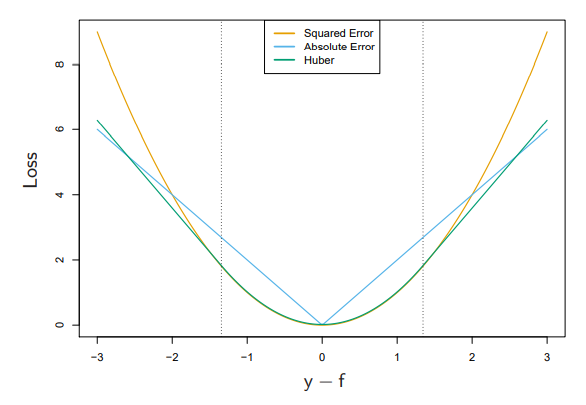
\includegraphics[width=0.7\linewidth]{_pictures/huber_loss} 

}

\caption{Comparison of different regression loss functions.}\label{fig:lossComp}
\end{figure}

These alternative loss criteria are more robust but make the fitting i.e.~the minimization much more complex as they do not yield such simplifications like the \(L_2\) loss.\citep{elements} The next step in the journey of exploring boosting is to narrow down the argument spaces of \textbf{Algorithm 1} (Forward Stagewise Additive Modeling) and to specify a subset of the general space of learning algorithms. This subset will be the space of Classification and Regression Tree (CART) models and in this case as the focus is on a regression task the space of regression trees. This choice is by no means arbitrary as in practice tree-based boosting algorithms have proven countless of times that they provide very robust and accurate models but still other learners might be chosen.\citep[\citet{HandsOnMLwithR}]{elements} The next subsection will explore how one can actually fit such a forward stagewise additive model when using regression trees as the learner class.

\hypertarget{general-gradient-tree-boosting}{%
\section{General gradient tree boosting}\label{general-gradient-tree-boosting}}

From now on there is the switch from the space of learning algorithms \(\mathcal{F}\) to the space of regression trees \(\mathcal{T}\). Such a regression tree can be formally expressed by:

\begin{equation}
  t(x, \gamma, R) = \sum_{j=1}^J \gamma_j I(x \in R_j) \quad \text{for  } t \in \mathcal{T}
  \label{eq:treeDef}
\end{equation}

With \(R_j\) being \(J\) distinct regions of the predictor space usually attained by recursive binary splitting. Moreover these regions correspond to the leafs of the tree and the number of leafs \(J\) or the depth of the trees are most often hyperparameters (not trained). The \(\gamma_j \in \mathbb{R}\) are the predictions for a given x if x is contained in the region \(R_j\). While it is quite easy to get the \(\gamma_j\) for the regions given, most often by computing \(\gamma_j = \frac{1}{|\{x \in R_j\}|} \sum_{\{x \in R_j\}} x\) , it is a much harder problem to get good distinct regions. The above mentioned recursive binary splitting is an approximation to do this and works in a top down greedy fashion.\citep{elements} From now on we assume that we have an efficient way of fitting such trees to a metric outcome variable e.g.~by recursive binary splitting.

A nice graphical example of an additive model based on trees is displayed in the figure \ref{fig:exampleAdditiveTree} below.\citep{xgboostPaper}

\begin{figure}

{\centering 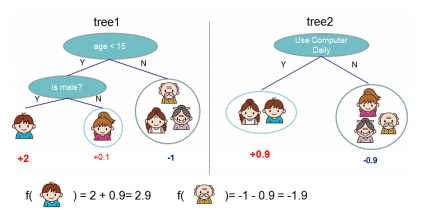
\includegraphics[width=0.7\linewidth]{_pictures/boosting_easy} 

}

\caption{Example of an additive tree ensamble.}\label{fig:exampleAdditiveTree}
\end{figure}

Having now the new space \(\mathcal{T}\) for the general boosting model \eqref{eq:additiveModel} one can write down the optimization problem that has to be solved in each step of the forward stagewise process of fitting the model.

\begin{equation}
  (\gamma^{(k)},R^{(k)}) = argmin_{\gamma,R} \sum_{i=1}^N L(y_i, \phi_{k-1}(x_i) + t(x_i,\gamma,R))
  \label{eq:oneStepTreeBoost}
\end{equation}

This can be estimated fast and quite straight forward if there is a simplification like the one seen for the \(L_2\) loss. But in the more general case of an arbitrary differentiable convex loss function like the Huber loss techniques from numerical optimization are needed to derive fast algorithms.\citep{elements}

\hypertarget{numOpt}{%
\subsection{Numerical optimization}\label{numOpt}}

According to \textbf{Algorithm 1} the goal in order to fit the boosting model is to minimize over the full loss of the training data \(\mathcal{D}\) which is the sum over all observation losses.

\[
L(\phi) = \sum_{i=1}^N L(y_i, \phi(x_i))
\]

And thus the \(\hat{\phi}\) additive boosting model we try to get is the following.

\[
\hat{\phi} = argmin_{\phi} L(\phi)
\]

Now we basically follow the spirit of the general gradient descent algorithm for differentiable functions. In the general case we minimize a function \(f(x)\) by stepping iteratively along the direction of the steepest descent i.e.~the negative gradient. The step length can then either be a constant small scalar or be determined by a line search.

In the setting of the additive boosting model \(\phi\) can be viewed as a vector of dimension \(N\) that contains the prediction according to \(\phi\) of the corresponding observation i.e.~\(\phi = (\phi(x_1),...,\phi(x_N))\). So the loss function \(L(\phi)\) corresponds to the \(f(x)\) in the general gradient descent algorithm. Numerical optimization, here gradient descent, then solves for \(\hat{\phi}\) by a sum of vectors of the same dimension as the \(\phi\).\citep{elements} The result of the sum \(\phi_K\) (\eqref{eq:numOptSol}) can be viewed as the current proposal for the optimal \(\hat{\phi}\) after \(K\) optimization steps and each \(h^{(k)}\) is the proposed improvement step.

\begin{equation}
  \phi_K = \sum_{k=0}^K h^{(k)} \quad h^{(k)} \in \mathbb{R}^N 
  \label{eq:numOptSol}
\end{equation}

While \(h^{(0)}\) is just an initial guess the subsequent \(h^{(k)}\) are again the prediction vectors of the corresponding model out of \(\mathcal{T}\) i.e.~\(h^{(k)}_{i} = t_k(x_i)\) with \(t \in \mathcal{T}\). This means that each \(\phi_k = \phi_{k-1} + h^{(k)}\). The \(h^{(k)}\) are calculated via the gradient which finally comes into play. As mentioned above one minimizes the loss the most by going towards the direction of the steepest descent. For \eqref{eq:numOptSol} follows from its additive formulation and defining \(g^{(k)}\) as the gradient of \(L(\phi_k)\) evaluated for \(\phi_{k-1}\) the update \(h^{(k)} = -\lambda_k g^{(k)}\). As we assumed the loss to be differentiable we see that \(g^{(k)}\) is well defined. Here \(\lambda_k\) is the usual step length for gradient descent methods. It is the solution of the line search \(\lambda_k = argmin_{\lambda} L(\phi_{k-1} - \lambda g^{(k)})\). This \(\lambda_k\) almost exactly corresponds to the \(\beta_k\) in \textbf{Algorithm 1} although here the optimization is performed for every region of the tree separately.\citep{elements}

With these insights it is clear that the tree predictions correspond to the negative gradient \(-g^{(k)}\). Of course the predictions are not independent as the prediction is constant for each leaf of the tree. So the new optimization proposed by numerical optimization via gradient boosting is given in \eqref{eq:oneStepTreeBoostnew} below.

\begin{equation}
  (\tilde{\gamma}^{(k)},\tilde{R}^{(k)}) = argmin_{\gamma,R} \sum_{i=1}^N [-g^{(k)}_{i} -  t(x_i,\gamma,R)] ^2
  \label{eq:oneStepTreeBoostnew}
\end{equation}

In words this just means fitting a regression tree by least squares to the negative gradients that were evaluated with the current predictions. The solution regions will not exactly match the ones from \eqref{eq:oneStepTreeBoost} but should be very similar.\citep{elements} After having estimated the regions one estimates the parameters \(\gamma\) by solving the line search \eqref{eq:gammaLineSearch}.

\begin{equation}
  \tilde{\gamma}^{(k)}_{j} = argmin_{\gamma^{(k)}_{j}} \sum_{x \in R^{(k)}_{j}} L(y_i,\phi_{k-1}(x_i) + \gamma^{(k)}_{j})
  \label{eq:gammaLineSearch}
\end{equation}

Putting all of this back together with \textbf{Algorithm 1} results in \textbf{Algorithm 2} that covers a general algorithm for tree-based gradient boosting.

\begin{center}\rule{0.5\linewidth}{0.5pt}\end{center}

\textbf{Algorithm 2}: Tree-based gradient boosting \citep{elements}

\begin{center}\rule{0.5\linewidth}{0.5pt}\end{center}

\begin{enumerate}
\def\labelenumi{\arabic{enumi}.}
\item
  Initialize \(\phi_0(x)\) as a singular node tree.
\item
  For \(k = 1\) to \(K\) do:

  \begin{itemize}
  \item
    For \(i = 1\) to \(N\) compute:

    \(g^{(k)}_{i} = \bigg[\frac{\partial L(y_i, \phi(x_i))}{\partial \phi(x_i)}\bigg]_{\phi = \phi_{k-1}}\)
  \item
    Fit a regression tree by least squares to the outcome vector \(-g^{(k)}\) in order to get the \(J^{(k)}\) distinct regions \(\tilde{R}^{(k)}_j\).
  \item
    For each of these \(J^{(k)}\) regions perform a line search in order to compute the leaf predictions \(\tilde{\gamma}^{(k)}_{j}\) exactly like in \eqref{eq:gammaLineSearch}.
  \item
    Set \(\phi_k(x) = \phi_{k-1}(x) + t(x,\tilde {\gamma}^{(k)}_{j},\tilde{R}^{(k)}_j)\) with \(t \in \mathcal{T}\)
  \end{itemize}
\end{enumerate}

\begin{center}\rule{0.5\linewidth}{0.5pt}\end{center}

The only unknowns in this algorithm are now the differentiable loss function and the hyperparameters like the \(J^{(k)}\) and the \(K\). While choices for the hyperparameters are discussed further below, the following table \ref{tab:lossGradients} displays the gradients for the losses discussed so far.

\begin{longtable}[]{@{}
  >{\raggedright\arraybackslash}p{(\columnwidth - 2\tabcolsep) * \real{0.27}}
  >{\raggedright\arraybackslash}p{(\columnwidth - 2\tabcolsep) * \real{0.73}}@{}}
\caption{\label{tab:lossGradients} Gradients of the discussed losses \citep{elements}}\tabularnewline
\toprule
Loss & Gradient \\
\midrule
\endfirsthead
\toprule
Loss & Gradient \\
\midrule
\endhead
\(L_2\): \((y_i - \phi(x_i))^2\) & \(2(y_i - \phi(x_i))\) \\
\(L_1\): \(|y_i - \phi(x_i)|\) & \(sign(y_i - \phi(x_i))\) \\
Huber loss \eqref{eq:huberLoss} & \(y_i - \phi(x_i)\) for \(|y_i - \phi(x_i)| \leq \delta\)

\(\delta sign(y_i - \phi(x_i))\) otherwise, with \(\delta\) quantile of \(|y_i - \phi(x_i)|\) \\
\bottomrule
\end{longtable}

\hypertarget{single-tree-depth}{%
\subsection{Single tree depth}\label{single-tree-depth}}

The question which \(J^{(k)}\) should be used at each iteration is now shortly discussed. Basically using the tree depth two means allowing only the main effects and no interactions. A value of 3 already allows all two way interaction effects and so on. As one stacks these models additive and does not restrict oneself to a single one, the building of a large tree and then pruning it back at each iteration as the regular CART algorithms do would be a computational overkill. Instead it has proven to be sufficient and efficient in practice to set the values \(J^{(k)}\) to a constant \(J \approx 6\).\citep{elements} Also decision stumps (\(J = 2\)) could be used but may require a lot more iterations.

\hypertarget{combOver}{%
\subsection{Combat overfitting}\label{combOver}}

No learning algorithm could be fully covered without treating the good old problem of overfitting. In the setting of boosting the experienced eye could have spotted the problem of overfitting already in the definition of the additive model \eqref{eq:additiveModel}. There the number \(K\) of models that form the ensemble was introduced but was not discussed further till now. Of course one can arbitrarily fit or better say remember some given training data in order to minimize the loss with such an additive model by letting \(K\) be arbitrarily large. This comes from the fact that the loss reduces usually after each iteration over \(K\).\citep{elements} The easiest way to prevent overfitting is to have a validation set at hand which is disjoint from the training data. Having such a validation set at hand can be used to monitor the loss on the unseen data. In the case the loss would rise again on the validation data one can consider to stop the algorithm and to use the current iteration number for the final parameter \(K\). This approach is often called early stopping. Besides that there are methods that regularize the individual trees that are fitted in each iteration. Two of those will be discussed now.

\hypertarget{shrinkage}{%
\subsubsection{Shrinkage}\label{shrinkage}}

Shrinkage basically refers to just introducing a learning rate \(\eta\). This learning rate \(\eta\) scales the contribution of the new model. In general the learning rate should be in \((0,1]\) but in practice it has been shown that rather small values like \(\eta < 0.1\) work very good.\citep{elements} As almost everything in life this does not come for free. A smaller learning rate usually comes with a computational cost as with lower \(\eta\) a larger \(K\) is required. Those two hyperparameters represent a trade-off in a way. In practice it is advisable to use a small learning rate \(\eta\) and adjust the \(K\) accordingly which in this case would mean to make the \(K\) large enough until one reaches an early stopping point. Still it is good to keep in mind that a \(\eta\) that is too small can lead to an immense and unnecessary computational effort. All in all using shrinkage the update step in \textbf{Algorithm 2} changes to the following.

\begin{equation}
  \phi_k(x) = \phi_{k-1}(x) + \eta * t(x,\tilde {\gamma}^{(k)}_{j},\tilde{R}^{(k)}_j)
  \label{eq:shrinkage}
\end{equation}

\hypertarget{subsampling}{%
\subsubsection{Subsampling}\label{subsampling}}

The other method to regularize the trees will be subsampling. There are two different kinds of subsampling. The first one is row-subsampling which basically means just using a random fraction of the training data in each iteration when fitting the new tree. Common values are \(\frac{1}{2}\) but for a larger training set the value can be chosen to be smaller. This does not only help to prevent overfitting and thus achieving a better predictive performance but reduces also the computational effort in each iteration.\citep{elements} The approach is very similar to the dropout technique in the setting of deep neural networks.

Moreover one can apply column-subsampling or feature-subsampling. Here only a fraction of the features or an explicit number of the features are used in each iteration. This is the exact same method and intention as the one applied in random forest models. Again the technique not only boosts performance on unseen data but also reduces the computational time.\citep{xgboostPaper} Still it must be noted that by using one or both subsampling methods one introduces one or two additional hyperparameters to the model that have to be tuned.

Having the \textbf{Algorithm 2} for tree-based gradient boosting alongside some regularization techniques it is time to look at a very popular, efficient and powerful open source implementation.

\hypertarget{xgboost-a-highly-efficient-implementation}{%
\section{XGBoost a highly efficient implementation}\label{xgboost-a-highly-efficient-implementation}}

The XGBoost algorithm is a highly scalable, efficient and successful implementation and optimization of \textbf{Algorithm 2} introduced by Chen and Guestrin in 2016.\citep[\citet{HandsOnMLwithR}]{xgboostPaper} It has gained a lot of spotlight when it was integral for many winning submissions at kaggle machine learning challenges. In the following the most important tweaks that are proposed to \textbf{Algorithm 2} are covered.

\hypertarget{regularized-loss}{%
\subsection{Regularized loss}\label{regularized-loss}}

Instead of just minimizing a convex and differentiable loss \(L\) XGBoost minimizes the following regularized loss.\citep{xgboostPaper}

\begin{equation}
  \begin{split}
  \mathcal{L}(\phi) = L(\phi) + \sum_{k=1}^K \Omega(t_k) \\
  \text{where } \Omega(t) = \nu J + \frac{1}{2} \lambda ||\gamma||^2 \quad t \in \mathcal{T}
  \end{split}
  \label{eq:regLoss}
\end{equation}

Here \(J\) and \(\gamma\) again parameterize the regression trees \(t \in \mathcal{T}\) as defined in \eqref{eq:treeDef}. As evident from the formula both hyperparameters \(\nu\) and \(\lambda\) favor when increased less complex models at each iteration. This is again a measure against overfitting.

This regularized objective leads to a slightly modified version of the minimization problem \eqref{eq:oneStepTreeBoost} that has to be solved in each iteration.

\begin{equation}
  (\gamma^{(k)},R^{(k)}) = argmin_{\gamma,R} \sum_{i=1}^N L(y_i, \phi_{k-1}(x_i) + t(x_i,\gamma,R)) + \Omega(t(x_i,\gamma,R))
  \label{eq:oneStepXGBoost}
\end{equation}

Instead of the first order approach, that has been introduced in \ref{numOpt}, XGBoost uses a second order approximation to further simplify the objective. This means that besides the first order gradient \(g^{(k)}\) of the loss function evaluated at \(\phi_{k-1}\) also the second order gradient \(z^{(k)}_i = \bigg[\frac{\partial^2 L(y_i, \phi(x_i))}{\partial^2 \phi(x_i)}\bigg]_{\phi = \phi_{k-1}}\) is used. By neglecting constants one reaches the approximate new objective below.\citep{xgboostPaper}

\begin{equation}
\begin{split}
  \tilde{\mathcal{L}}^{(k)} & = \sum_{i=1}^N [g^{(k)}_i t^{(k)}(x_i) + \frac{1}{2} t^{(k)}(x_i)^2] + \Omega(t^{(k)}) \\
  & = \sum_{j=1}^J [(\sum_{\{i|x_i \in R^{(k)}_j\}} g^{(k)}_i) \gamma^{(k)}_j + \frac{1}{2} (\sum_{\{i|x_i \in R^{(k)}_j\}} z^{(k)}_i + \lambda) (\gamma^{(k)}_j)^2 ] + \nu J
\end{split}
\label{eq:oneappStepXGBoost}
\end{equation}

This representation is used as it can be decomposed by the \(J\) leafs of the tree. One can then define an scoring function for split finding that only depends on \(g^{(k)}\) and \(z^{(k)}\).

\hypertarget{shrinkage-and-subsampling}{%
\subsection{Shrinkage and subsampling}\label{shrinkage-and-subsampling}}

As discussed above in \ref{combOver} shrinkage and subsampling are great ways to regularize the model and prevent overfitting. XGBoost implements both shrinkage and subsampling. XGBoost enables the user to use column as well as row subsampling. The authors claim that in practice column subsampling has prevented overfitting more than row subsampling.\citep{xgboostPaper}

\hypertarget{even-more-tweaks}{%
\subsection{Even more tweaks}\label{even-more-tweaks}}

Besides the changes above the authors also implemented an effective approximate algorithm for split finding for the tree building step. A very nice attribute of this approximate procedure is that the algorithm is sparsity aware i.e.~the processing of missing values or 0 values is very efficient. This is done via a learned default direction in each split. Moreover they used very efficient data structures to allow a lot of parallel processing.\citep{xgboostPaper} It is written in C++ but has APIs in various languages like in R via the \texttt{xgboost} package.\citep{xgboost_package}

\hypertarget{hyperparameters-overview}{%
\subsection{Hyperparameters overview}\label{hyperparameters-overview}}

As the \textbf{tidymodels} framework will be used in the applied part, the according names from the parsnip interface for tree-based boosting i.e.~\texttt{boost\_tree} are discussed below.\citep[\citet{xgboost_package}, \citet{tidymodels}]{xgboostPaper}

\begin{longtable}[]{@{}
  >{\raggedright\arraybackslash}p{(\columnwidth - 4\tabcolsep) * \real{0.15}}
  >{\raggedright\arraybackslash}p{(\columnwidth - 4\tabcolsep) * \real{0.13}}
  >{\raggedright\arraybackslash}p{(\columnwidth - 4\tabcolsep) * \real{0.72}}@{}}
\caption{\label{tab:xgboostHyper} XGBoost hyperparameters overview.}\tabularnewline
\toprule
Hyperparameter & Notation above & Meaning \\
\midrule
\endfirsthead
\toprule
Hyperparameter & Notation above & Meaning \\
\midrule
\endhead
\texttt{trees} & \(K\) & Number of trees in the ensemble. \\
\texttt{tree\_depth} & \(max(J^{(k)})\) & Maximum depth of the trees. \\
\texttt{learn\_rate} & \(\eta\) & Learning rate (shrinkage). \\
\texttt{min\_n} & & Minimum number of observations in terminal region \(R^{(k)}_j\). \\
\texttt{lambda} & \(\lambda\) & \(L_2\) regularization parameter on \(\gamma\) as in \eqref{eq:oneappStepXGBoost} (default = 0). \\
\texttt{alpha} & & \(L_1\) regularization parameter on \(\gamma\) (default = 0). \\
\texttt{loss\_reduction} & \(\nu\) & Minimal loss reduction for terminal partitions. (default = 0) \\
\texttt{mtry} & & Proportion or number of columns for column subsampling. \\
\texttt{sample\_size} & & Proportion of observations for row subsampling. \\
\texttt{stop\_iter} & & Allowed number of rounds without improvement before early stopping. \\
\bottomrule
\end{longtable}

Note that the \(L_1\) penalization term would be added to the \(\Omega\) term in the loss \(\mathcal{L}\) of XGBoost.

This closes the chapter on the theory of boosting methods with a focus on tree-based gradient boosting. The discussed tools will be put to the test in the subsequent sections where real world data will be analyzed with them.

\hypertarget{eda}{%
\chapter{Explore the data}\label{eda}}

Before one starts with the actual modeling it is crucial to get to know the data and to bring it to the correct format. This process of getting familiar with the data is well known as Exploratory Data Analysis (EDA). To do this many packages are used.\citetext{\citealp{tidyverse}; \citealp{tidymodels}; \citealp{viridis}; \citealp{ggtext}; \citealp[ ]{viridisLite}; \citealp{patchwork}; \citealp{visdat}; \citealp{lubridate}} The most important ones will be loaded below.

\begin{Shaded}
\begin{Highlighting}[]
\FunctionTok{library}\NormalTok{(tidyverse) }\CommentTok{\# general data handling tools}
\FunctionTok{library}\NormalTok{(tidymodels) }\CommentTok{\# data modeling and preprocessing}
\CommentTok{\# color palettes}
\FunctionTok{library}\NormalTok{(viridis)}
\FunctionTok{library}\NormalTok{(viridisLite)}
\FunctionTok{library}\NormalTok{(patchwork) }\CommentTok{\# composing of ggplots}
\end{Highlighting}
\end{Shaded}

\hypertarget{burnout-data}{%
\section{Burnout data}\label{burnout-data}}

The data is from the machine learning challenge \emph{HackerEarth Machine Learning Challenge: Are your employees burning out?}. And can be downloaded here: \url{https://www.kaggle.com/blurredmachine/are-your-employees-burning-out?select=train.csv}

\begin{Shaded}
\begin{Highlighting}[]
\CommentTok{\# load the data}
\NormalTok{burnout\_data }\OtherTok{\textless{}{-}} \FunctionTok{read\_csv}\NormalTok{(}\StringTok{"\_data/burn\_out\_train.csv"}\NormalTok{)}
\CommentTok{\# convert colnames to snake\_case}
\FunctionTok{colnames}\NormalTok{(burnout\_data) }\OtherTok{\textless{}{-}} \FunctionTok{tolower}\NormalTok{(}
\NormalTok{  stringr}\SpecialCharTok{::}\FunctionTok{str\_replace\_all}\NormalTok{(}
    \FunctionTok{colnames}\NormalTok{(burnout\_data),}
    \StringTok{" "}\NormalTok{,}
    \StringTok{"\_"}
\NormalTok{  ))}
\CommentTok{\# omit missing values in the outcome variable}
\NormalTok{burnout\_data }\OtherTok{\textless{}{-}}\NormalTok{ burnout\_data[}\SpecialCharTok{!}\FunctionTok{is.na}\NormalTok{(burnout\_data}\SpecialCharTok{$}\NormalTok{burn\_rate),]}
\end{Highlighting}
\end{Shaded}

\hypertarget{train-test-split}{%
\subsection{Train-test split}\label{train-test-split}}

\begin{Shaded}
\begin{Highlighting}[]
\FunctionTok{set.seed}\NormalTok{(}\DecValTok{2}\NormalTok{)}
\NormalTok{burnout\_split }\OtherTok{\textless{}{-}}\NormalTok{ rsample}\SpecialCharTok{::}\FunctionTok{initial\_split}\NormalTok{(burnout\_data, }\AttributeTok{prop =} \FloatTok{0.80}\NormalTok{)}
\NormalTok{burnout\_train }\OtherTok{\textless{}{-}}\NormalTok{ rsample}\SpecialCharTok{::}\FunctionTok{training}\NormalTok{(burnout\_split)}
\NormalTok{burnout\_test  }\OtherTok{\textless{}{-}}\NormalTok{ rsample}\SpecialCharTok{::}\FunctionTok{testing}\NormalTok{(burnout\_split)}
\end{Highlighting}
\end{Shaded}

The training data set contains 17301 rows and 9 variables.

The test data set contains 4325 observations and naturally also 9 variables.

\hypertarget{quick-general-overview}{%
\subsection{Quick general overview}\label{quick-general-overview}}

First look at the classes of the variables.

\begin{tabular}{l|l}
\hline
column & class\\
\hline
employee\_id & character\\
\hline
date\_of\_joining & Date\\
\hline
gender & character\\
\hline
company\_type & character\\
\hline
wfh\_setup\_available & character\\
\hline
designation & numeric\\
\hline
resource\_allocation & numeric\\
\hline
mental\_fatigue\_score & numeric\\
\hline
burn\_rate & numeric\\
\hline
\end{tabular}

A general visualization to detect missing values.

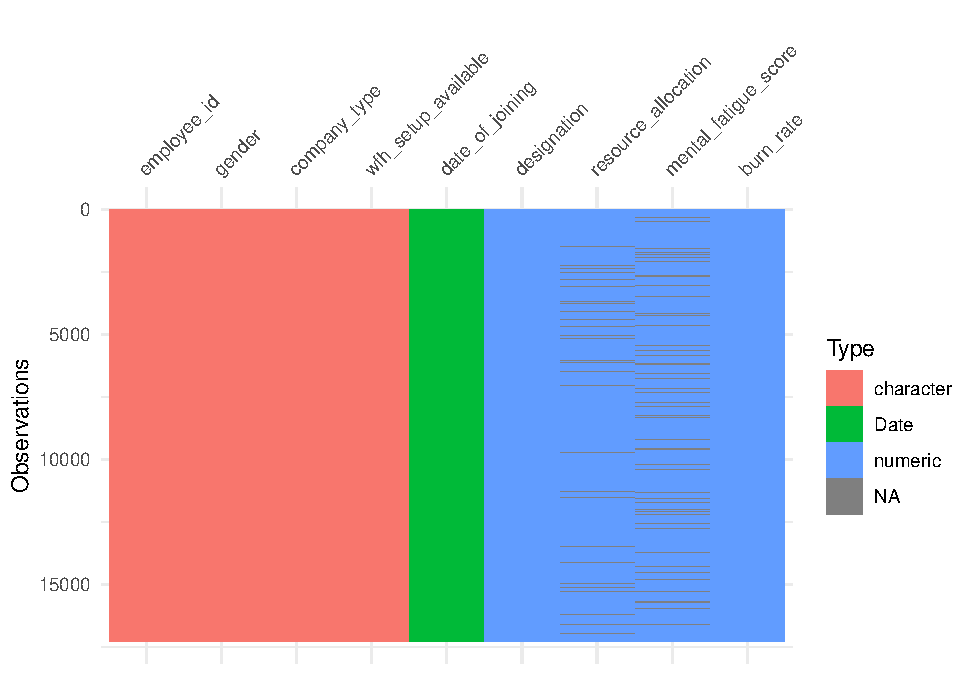
\includegraphics{boosting_methods_files/figure-latex/visdat-1.pdf}

\begin{Shaded}
\begin{Highlighting}[]
\CommentTok{\# percentage of missing values in the training data set}
\FunctionTok{mean}\NormalTok{(}\FunctionTok{rowSums}\NormalTok{(}\FunctionTok{is.na}\NormalTok{(burnout\_train)) }\SpecialCharTok{\textgreater{}} \DecValTok{0}\NormalTok{)}
\end{Highlighting}
\end{Shaded}

\begin{verbatim}
## [1] 0.1407433
\end{verbatim}

As we know that XGBoost can handle missing values we do not have to be concerned. Although one can think about imputation. But more on that later.

\hypertarget{what-about-the-outcome-variable}{%
\subsection{What about the outcome variable?}\label{what-about-the-outcome-variable}}

\texttt{burn\_rate}: For each employee telling the rate of burnout should be in \([0,1]\). The greater the score the worse the burnout (0 means no burnout at all). As the variable is continuous we have a regression task. Yet it has bounds which has to be treated with when predicting.

The five point summary below shows that the full range is covered and no invalid values are in the data.

\begin{verbatim}
##    Min. 1st Qu.  Median    Mean 3rd Qu.    Max. 
##  0.0000  0.3100  0.4500  0.4513  0.5900  1.0000
\end{verbatim}

Now the distribution of the outcome.

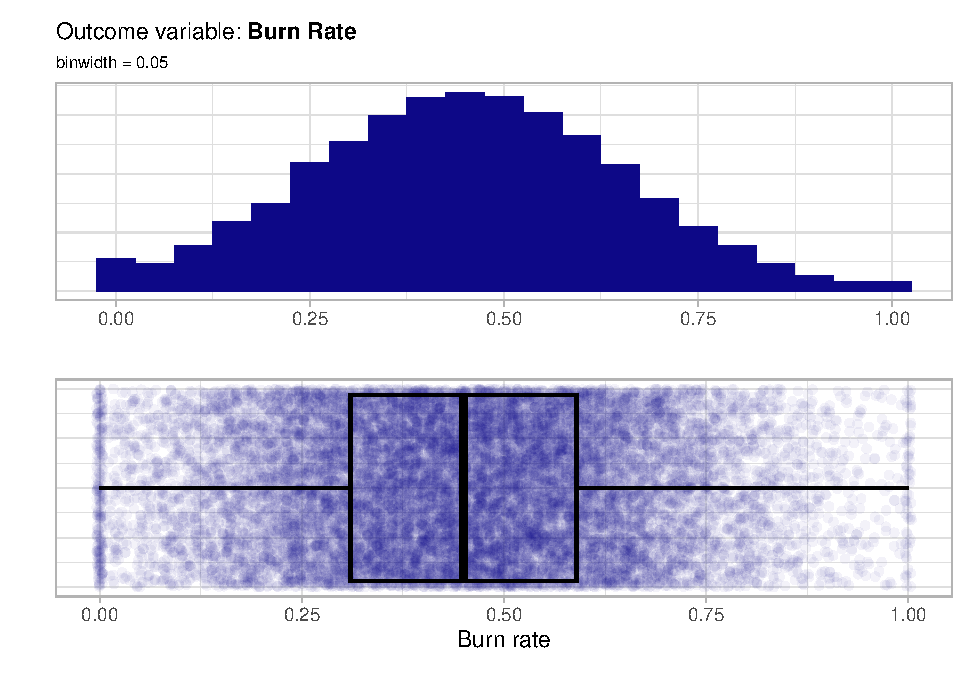
\includegraphics{boosting_methods_files/figure-latex/unnamed-chunk-5-1.pdf}

The distribution of the outcome is very much symmetrical and bell shaped around 0.5 and the whole defined region \([0,1]\) is covered quite well.

\hypertarget{distribution-and-main-effects-of-the-predictors}{%
\subsection{Distribution and main effects of the predictors}\label{distribution-and-main-effects-of-the-predictors}}

\hypertarget{employee-id}{%
\subsubsection{Employee ID}\label{employee-id}}

\texttt{employee\_id} is just an ID variable and thus is not useful for any prediction model. But one has to check for duplicates.

\begin{Shaded}
\begin{Highlighting}[]
\CommentTok{\# TRUE if there are NO duplicates}
\NormalTok{burnout\_train }\SpecialCharTok{\%\textgreater{}\%}
  \FunctionTok{group\_by}\NormalTok{(employee\_id) }\SpecialCharTok{\%\textgreater{}\%}
  \FunctionTok{summarise}\NormalTok{(}\AttributeTok{n =} \FunctionTok{n}\NormalTok{()) }\SpecialCharTok{\%\textgreater{}\%}
  \FunctionTok{nrow}\NormalTok{() }\SpecialCharTok{==} \FunctionTok{nrow}\NormalTok{(burnout\_train)}
\end{Highlighting}
\end{Shaded}

\begin{verbatim}
## [1] TRUE
\end{verbatim}

Thus there are no duplicates which is good.

\hypertarget{date-of-joining}{%
\subsubsection{Date of joining}\label{date-of-joining}}

\texttt{date\_of\_joining} is the date the employee has joined the company. Thus a continuous variable that most likely needs some kind of feature engineering.

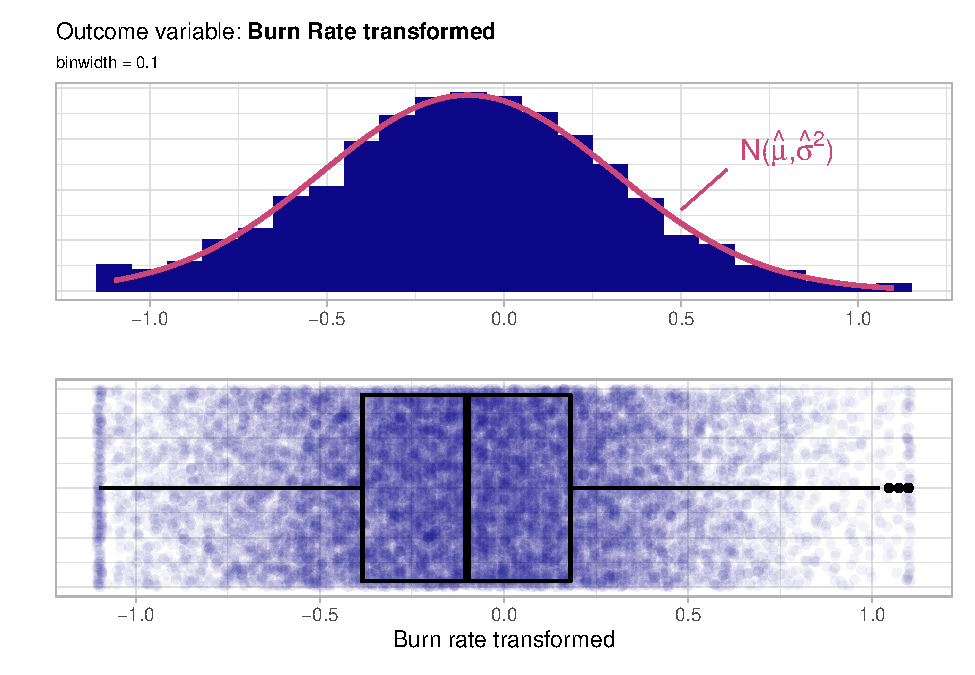
\includegraphics{boosting_methods_files/figure-latex/unnamed-chunk-7-1.pdf}

Although there is a lot of variation no major trends in hirings are visible from this plot. Overall the variable seems to be quite equally distributed over the year 2008.

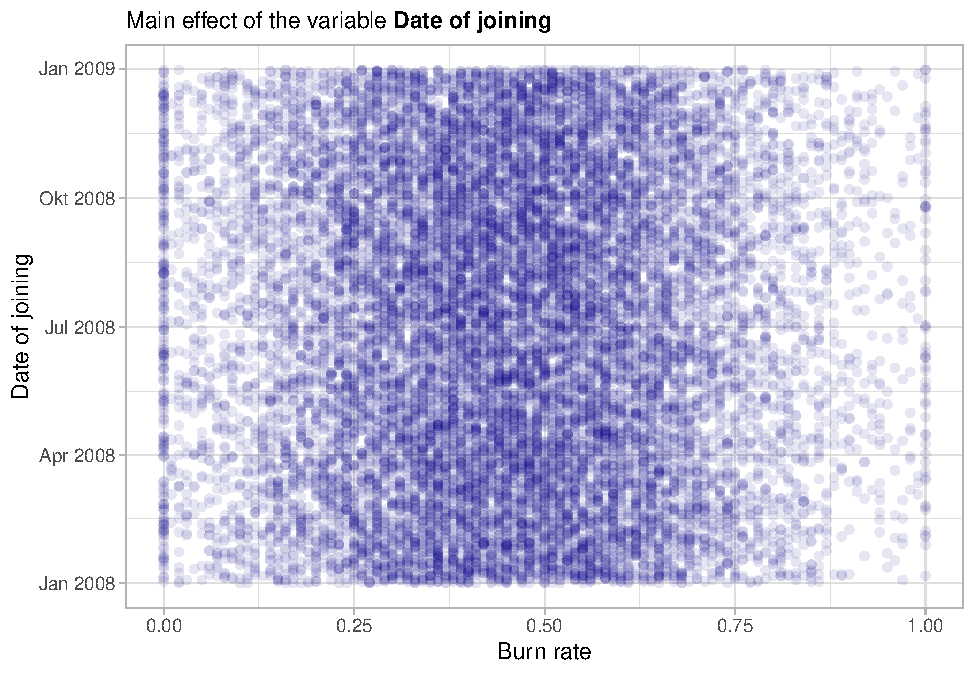
\includegraphics{boosting_methods_files/figure-latex/unnamed-chunk-8-1.pdf}

In its raw form the variable \texttt{date\_of\_joining} seems not to have a notable main effect on the outcome variable. Nevertheless the feature will be used in the model and as tree-based models have an in-built feature selection one can see after the fitting if the feature was helpful overall. The feature will not be included just as an integer (the default format how Dates are represented) but rather some more features like weekday or month will be extracted from the raw variable further down the road.

\hypertarget{gender}{%
\subsubsection{Gender}\label{gender}}

\texttt{gender} represents the gender of the employee. Definitely a categorical variable.

\begin{Shaded}
\begin{Highlighting}[]
\CommentTok{\# have a look at the discrete distribution}
\FunctionTok{summary}\NormalTok{(}\FunctionTok{factor}\NormalTok{(burnout\_train}\SpecialCharTok{$}\NormalTok{gender))}
\end{Highlighting}
\end{Shaded}

\begin{verbatim}
## Female   Male 
##   9101   8200
\end{verbatim}

The two classes are well balanced. Now a look at the main effect of the feature.

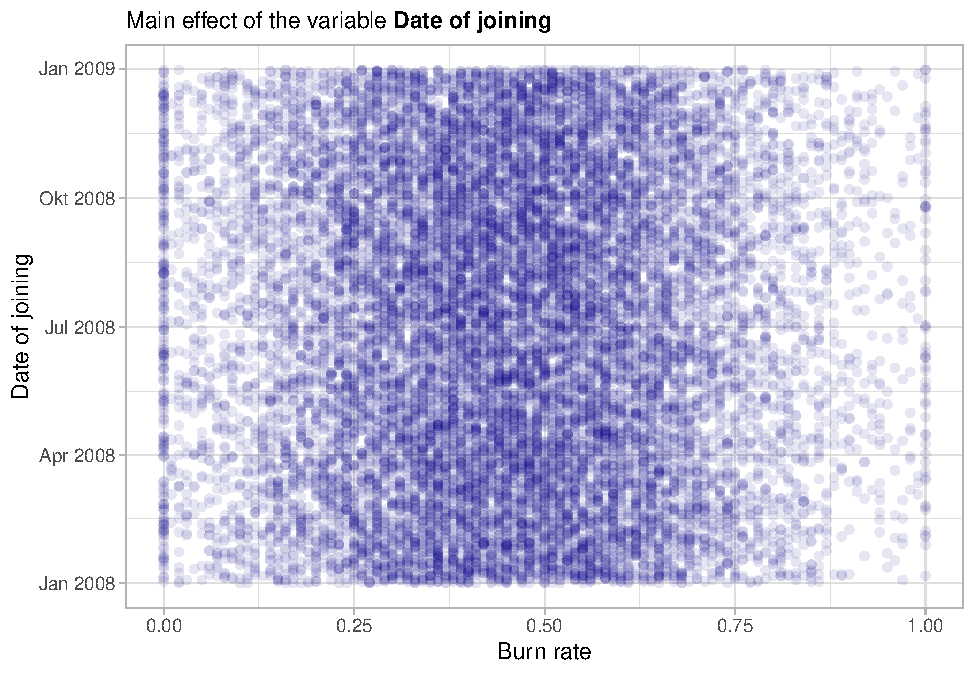
\includegraphics{boosting_methods_files/figure-latex/unnamed-chunk-10-1.pdf}

For both classes the distributions are very similar and symmetrical. It seems like the male employees have overall a slightly higher risk of having a higher burn score i.e.~a burnout.

\hypertarget{company-type}{%
\subsubsection{Company type}\label{company-type}}

\texttt{company\_type} is a binary categorical variable that indicates whether the company is a service or product company.

\begin{Shaded}
\begin{Highlighting}[]
\CommentTok{\# have a look at the discrete distribution}
\FunctionTok{summary}\NormalTok{(}\FunctionTok{factor}\NormalTok{(burnout\_train}\SpecialCharTok{$}\NormalTok{company\_type))}
\end{Highlighting}
\end{Shaded}

\begin{verbatim}
## Product Service 
##    6018   11283
\end{verbatim}

In this case the classes are not fully balanced but each class is still well represented. Now a look at the main effect of the feature.

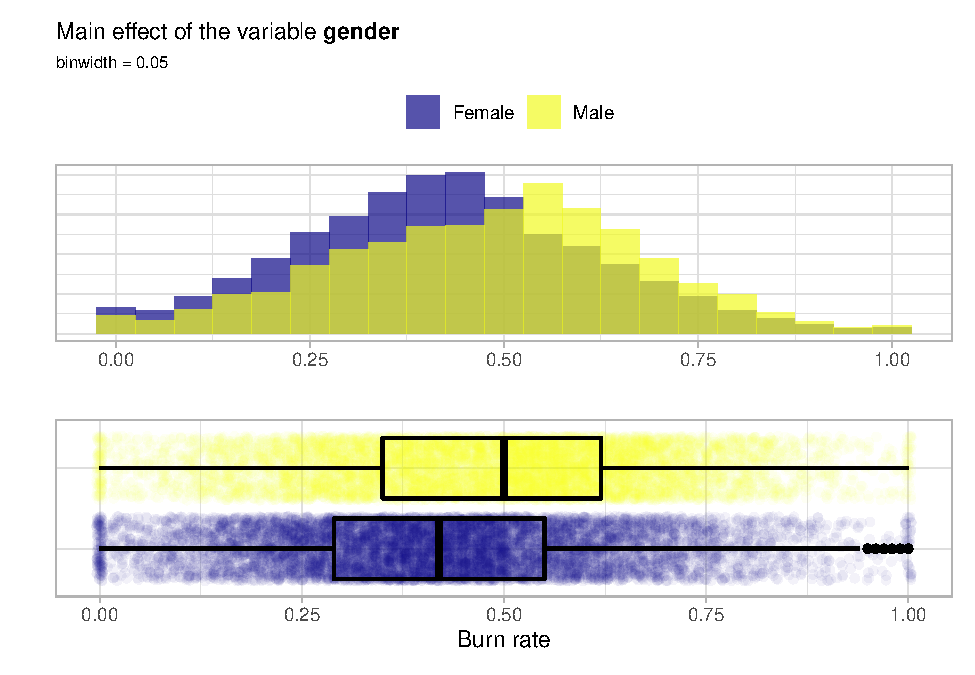
\includegraphics{boosting_methods_files/figure-latex/unnamed-chunk-12-1.pdf}

For both classes the distributions are almost identical and symmetrical. From an univariate point of view no notable main effect is visible from these visualizations.

\hypertarget{work-from-home-setup}{%
\subsubsection{Work from home setup}\label{work-from-home-setup}}

\texttt{wfh\_setup\_available} indicates whether a working from home setup is available for the employee. So this is again a binary variable.

\begin{Shaded}
\begin{Highlighting}[]
\CommentTok{\# have a look at the discrete distribution}
\FunctionTok{summary}\NormalTok{(}\FunctionTok{factor}\NormalTok{(burnout\_train}\SpecialCharTok{$}\NormalTok{wfh\_setup\_available))}
\end{Highlighting}
\end{Shaded}

\begin{verbatim}
##   No  Yes 
## 7929 9372
\end{verbatim}

The two classes are well balanced. Now a look at the main effect of the feature.

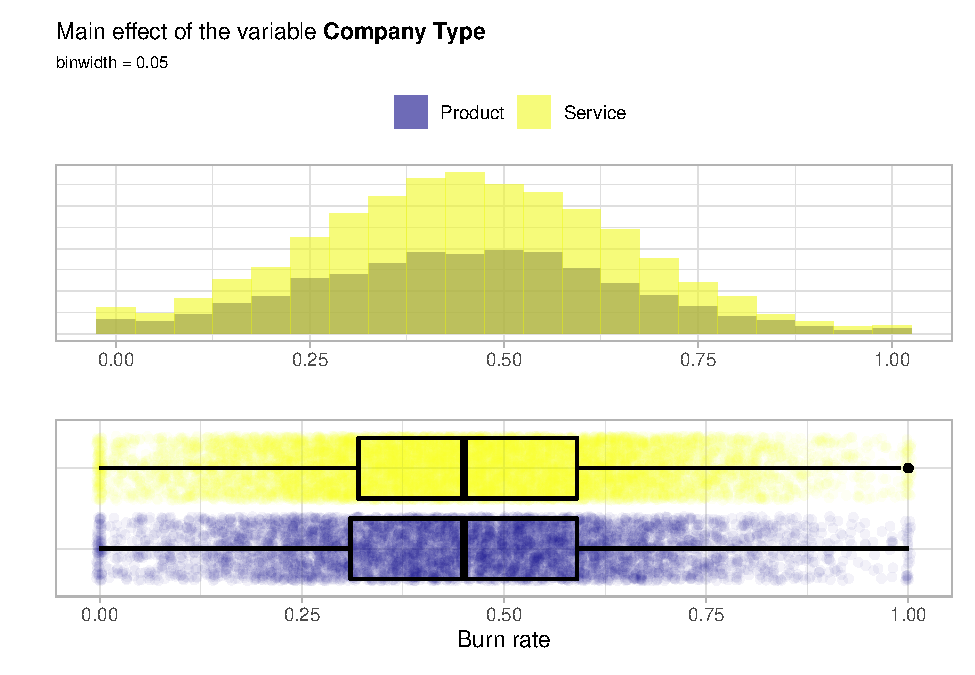
\includegraphics{boosting_methods_files/figure-latex/unnamed-chunk-14-1.pdf}

Again both distributions are quite similar i.e.~bell shaped and symmetrical. Here quite a main effect is visible. A work from home setup most likely has a positive influence on the wellbeing and thus lowers the risk for a high burn rate.

\hypertarget{designation}{%
\subsubsection{Designation}\label{designation}}

\texttt{designation} A rate within \([0,5]\) that represents the designation in the company for the employee. High values indicate a greater amount of designation.

\begin{Shaded}
\begin{Highlighting}[]
\CommentTok{\# unique values of the feature}
\FunctionTok{unique}\NormalTok{(burnout\_train}\SpecialCharTok{$}\NormalTok{designation)}
\end{Highlighting}
\end{Shaded}

\begin{verbatim}
## [1] 2 1 3 0 4 5
\end{verbatim}

As the feature has a natural ordering this variable will be treated as an ordinal one i.e.~be encoded with the integers and not by one-hot-encoding.

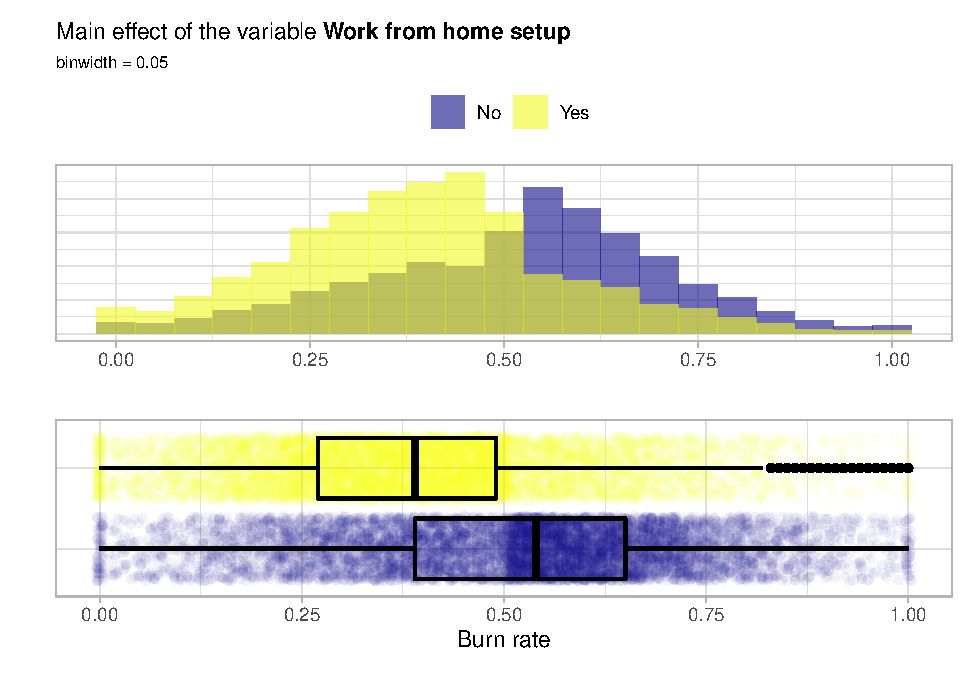
\includegraphics{boosting_methods_files/figure-latex/unnamed-chunk-16-1.pdf}

Here clearly the more extreme levels of designation are less represented in the data. This makes total sense w.r.t. the meaning of the variable.

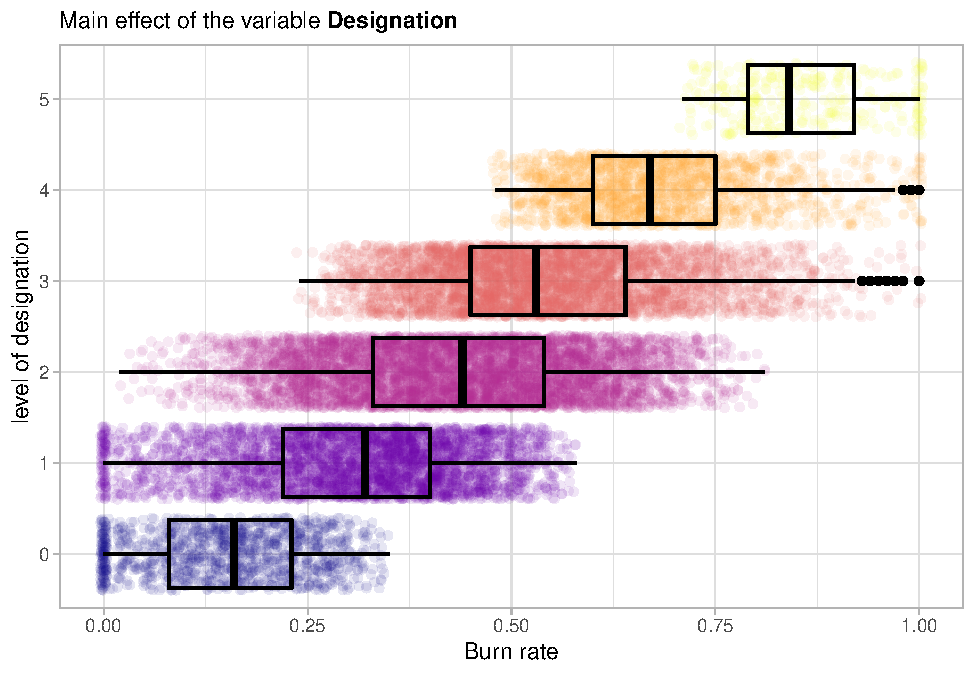
\includegraphics{boosting_methods_files/figure-latex/unnamed-chunk-17-1.pdf}

A strong main effect is visible in the plot. The plot also further strengthens the hypothesis that we should treat the feature as ordinal. A higher level of designation seems to have an influence on the risk of having a burnout. For example employees from the training data set with a level of designation below 3 never even achieved a maximal burn score of one.

\hypertarget{resource-allocation}{%
\subsubsection{Resource allocation}\label{resource-allocation}}

\texttt{resource\_allocation} A rate within \([1,10]\) that represents the resource allocation to the employee. High values indicate more resources allocated to the employee.

\begin{Shaded}
\begin{Highlighting}[]
\CommentTok{\# unique values of the feature}
\FunctionTok{unique}\NormalTok{(burnout\_train}\SpecialCharTok{$}\NormalTok{resource\_allocation)}
\end{Highlighting}
\end{Shaded}

\begin{verbatim}
##  [1]  3  1  7  4  6  5  2 NA  8 10  9
\end{verbatim}

Here again the question is whether one should encode this variable as a categorical or an ordinal categorical feature. In this case as there are quite some levels and again a natural ordering the variable will be encoded as a continuous integer score.

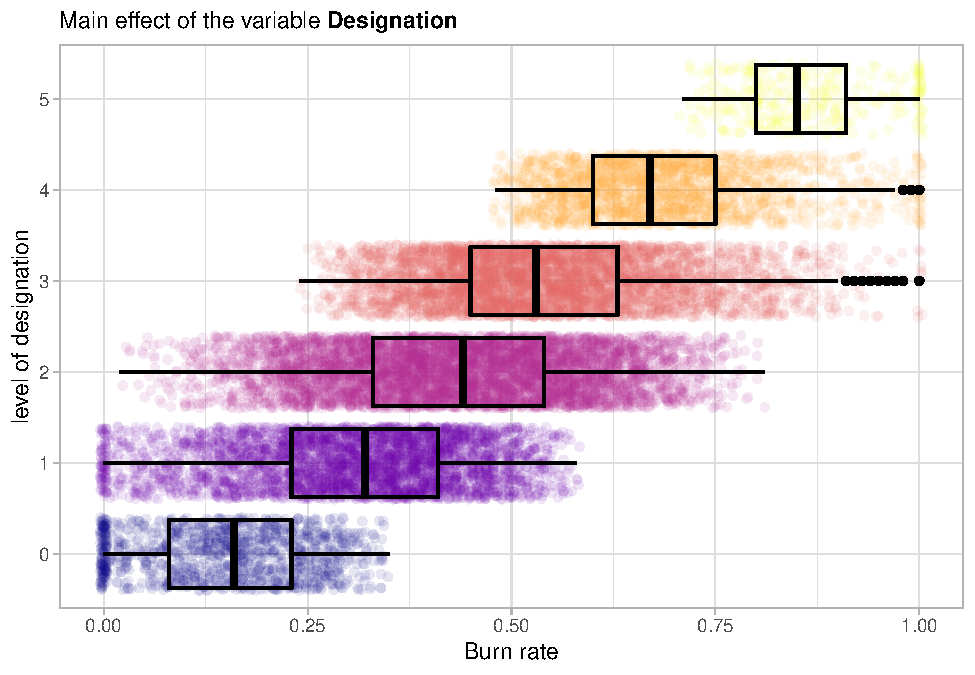
\includegraphics{boosting_methods_files/figure-latex/unnamed-chunk-19-1.pdf}

A similar behavior as the one of the previous variable is visible. But here there are some missing values (NA's).

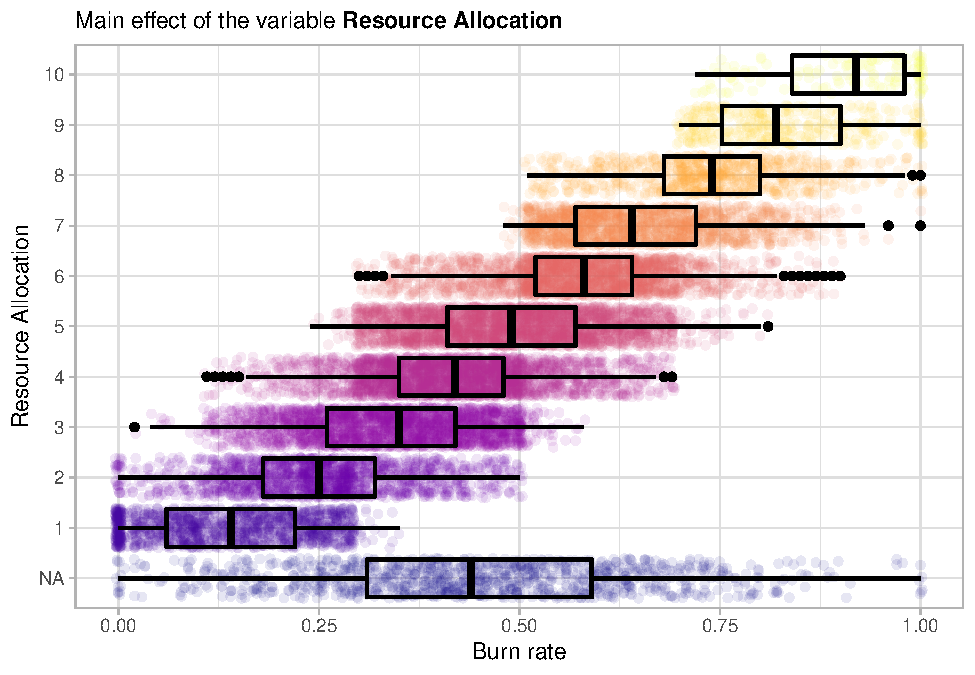
\includegraphics{boosting_methods_files/figure-latex/unnamed-chunk-20-1.pdf}

A strong main effect is visible in the plot. The plot again further strengthens the hypothesis that we should treat this feature as ordinal. A higher amount of resources assigned to an employee seems to have a positive influence on the risk of having a burnout. The missing values do not seem to have some structure as they replicate the base distribution of the outcome variable.

\hypertarget{mental-fatigue-score}{%
\subsubsection{Mental fatigue score}\label{mental-fatigue-score}}

\texttt{mental\_fatigue\_score} is the level of mental fatigue the employee is facing.

\begin{Shaded}
\begin{Highlighting}[]
\CommentTok{\# number of unique values}
\FunctionTok{length}\NormalTok{(}\FunctionTok{unique}\NormalTok{(burnout\_train}\SpecialCharTok{$}\NormalTok{mental\_fatigue\_score)) }
\end{Highlighting}
\end{Shaded}

\begin{verbatim}
## [1] 102
\end{verbatim}

This variable will without a question be treated in a continuous way.

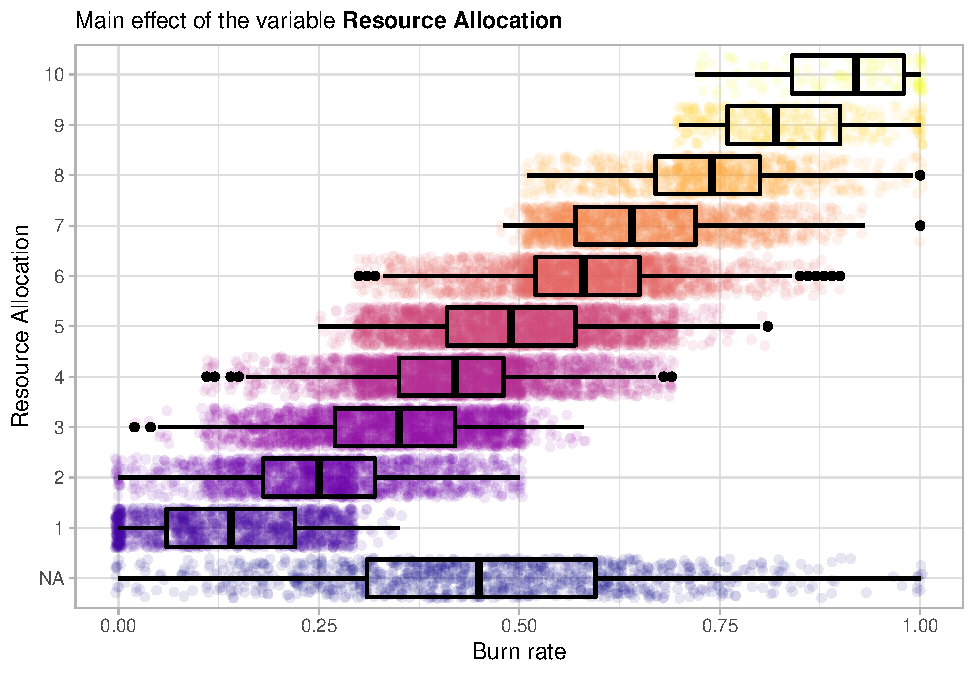
\includegraphics{boosting_methods_files/figure-latex/unnamed-chunk-22-1.pdf}

Although there is a very slight skew towards a higher mental fatigue score the overall distribution is still more or less bell shaped and quite symmetrical. Moreover the whole allowed range is covered and the bounds are not violated. Next the main effect of the variable.

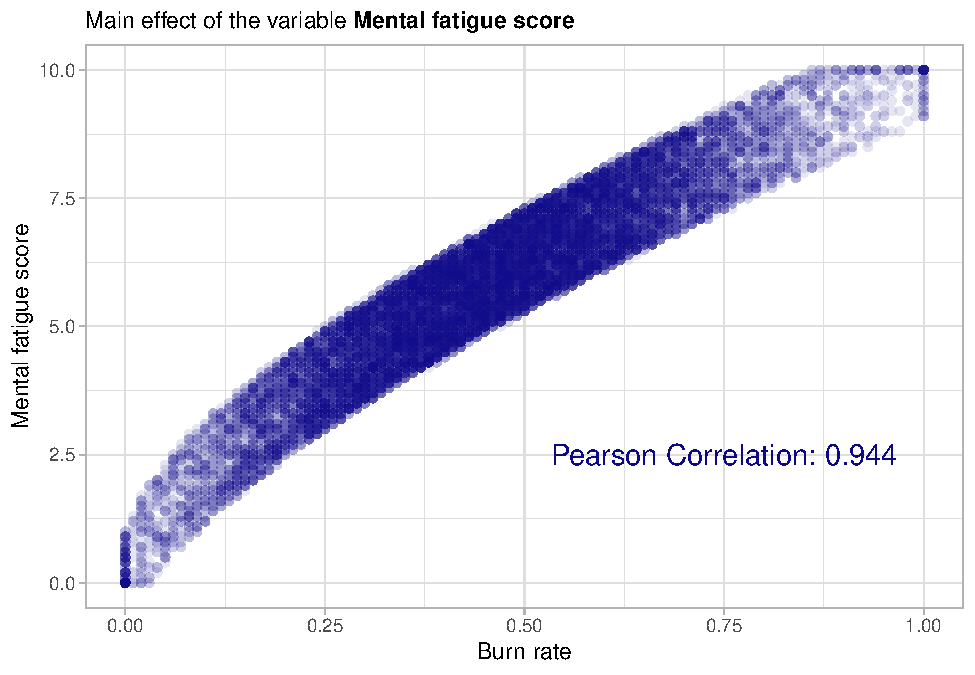
\includegraphics{boosting_methods_files/figure-latex/unnamed-chunk-23-1.pdf}

This scatterplot shows drastic results! The mental fatigue score has an almost perfect linear relationship with the outcome variable. This is also underlined by the very high pearson correlation. This indicates that mental fatigue score will be a most important predictor. If a communication with the data collector would be possible it would be important to check whether the two scores have common confounding variables as then one would have to question the practical usability of this predictor. This comes from the fact that no model would be needed if it was as hard to collect the data about the predictors as the outcome data. Moreover there are 1555 missing values in the feature so for those the model has to rely on the other maybe more weak predictors. It should be noted that when evaluating the final model one should consider to compare its performance to a trivial model (like a single intercept model). When constructing such a trivial model one could and maybe should also use this variable (when available) to get a trivial prediction by scaling the \texttt{mental\_fatigue\_score} feature by a simple scalar.

\hypertarget{relationships-between-the-predictors}{%
\subsection{Relationships between the predictors}\label{relationships-between-the-predictors}}

\hypertarget{date-of-joining-vs.-the-others}{%
\subsubsection{Date of joining vs.~the others}\label{date-of-joining-vs.-the-others}}

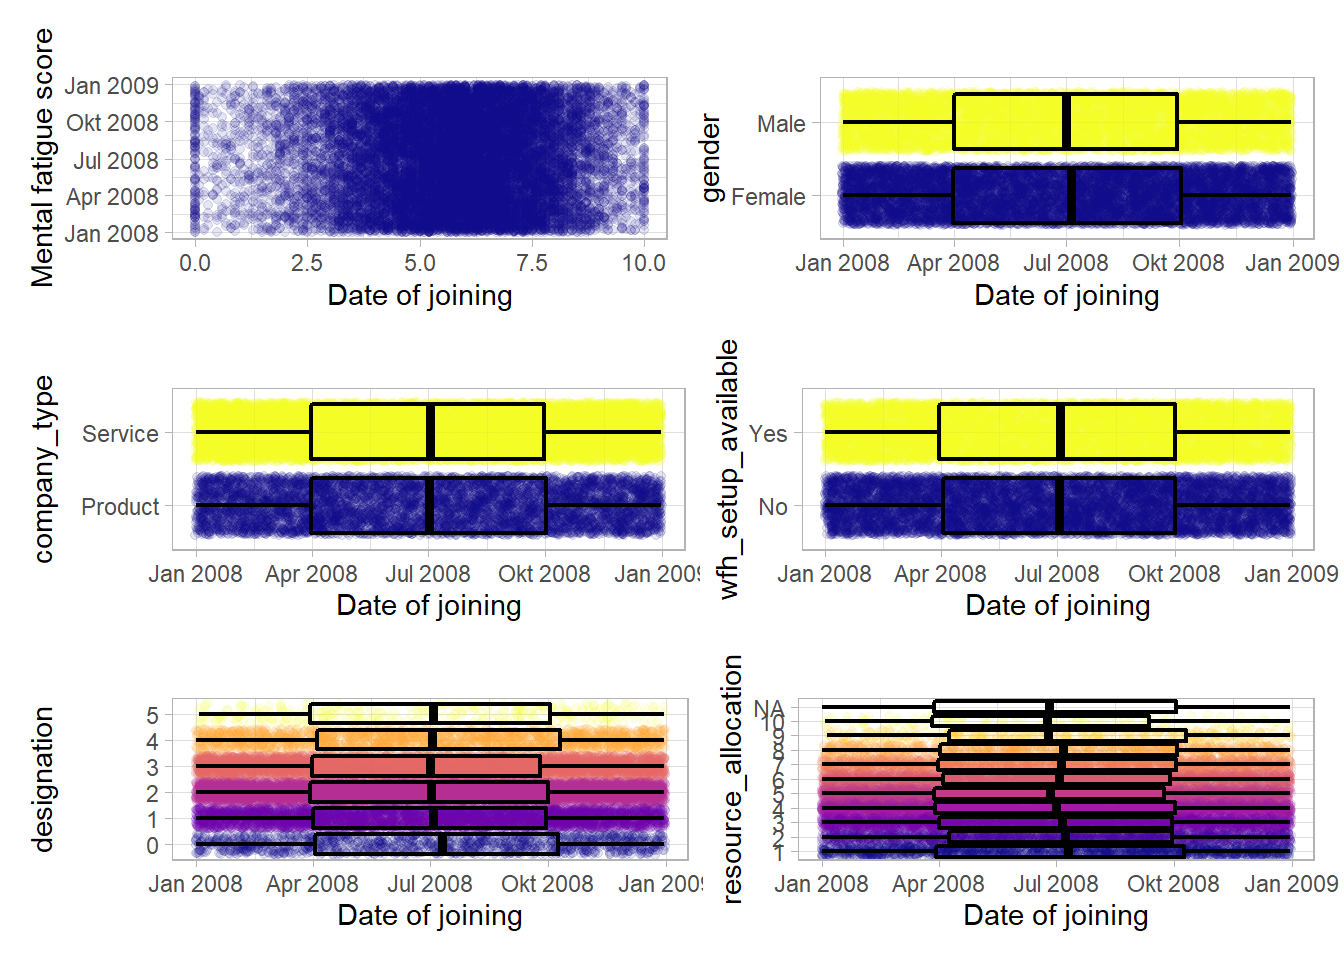
\includegraphics[width=0.9\linewidth]{boosting_methods_files/figure-latex/ggpairs-1}

No major relationship can be detected here.

\hypertarget{gender-vs.-the-remaining}{%
\subsubsection{Gender vs.~the remaining}\label{gender-vs.-the-remaining}}

\textbf{Contingency tables for the comparison of two binary features:}

\begin{Shaded}
\begin{Highlighting}[]
\CommentTok{\# Gender vs Company type}
\FunctionTok{table}\NormalTok{(burnout\_train}\SpecialCharTok{$}\NormalTok{gender, burnout\_train}\SpecialCharTok{$}\NormalTok{company\_type)}
\end{Highlighting}
\end{Shaded}

\begin{verbatim}
##         
##          Product Service
##   Female    3097    6004
##   Male      2921    5279
\end{verbatim}

No huge tendency visible.

\begin{Shaded}
\begin{Highlighting}[]
\CommentTok{\# Gender vs Work from home setup}
\FunctionTok{table}\NormalTok{(burnout\_train}\SpecialCharTok{$}\NormalTok{gender, burnout\_train}\SpecialCharTok{$}\NormalTok{wfh\_setup\_available)}
\end{Highlighting}
\end{Shaded}

\begin{verbatim}
##         
##            No  Yes
##   Female 3835 5266
##   Male   4094 4106
\end{verbatim}

Slightly more women have a work from home setup available.

\textbf{Now the ordinal variables:}

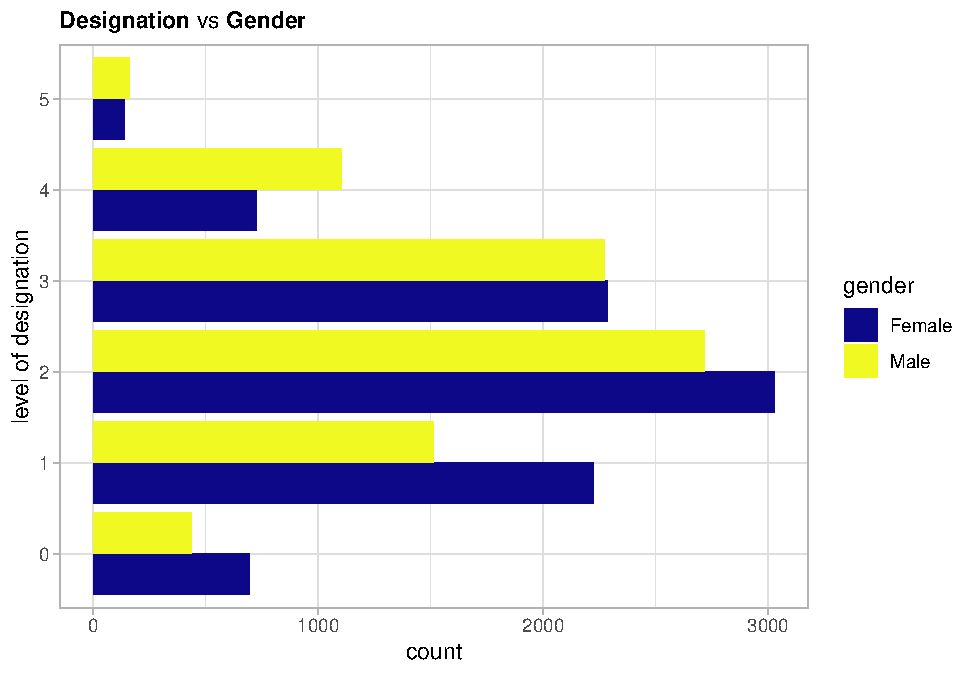
\includegraphics{boosting_methods_files/figure-latex/unnamed-chunk-27-1.pdf}

It has to be noted again that female and male emplyees are almost equally represented in the data set. Thus one can see from the above plot that the biggest difference in distribution is for the levels 1 and 4 with opposing effects. While male employees more often have a quite high designation of 4 females are the much more frequent employee with designation level 1.

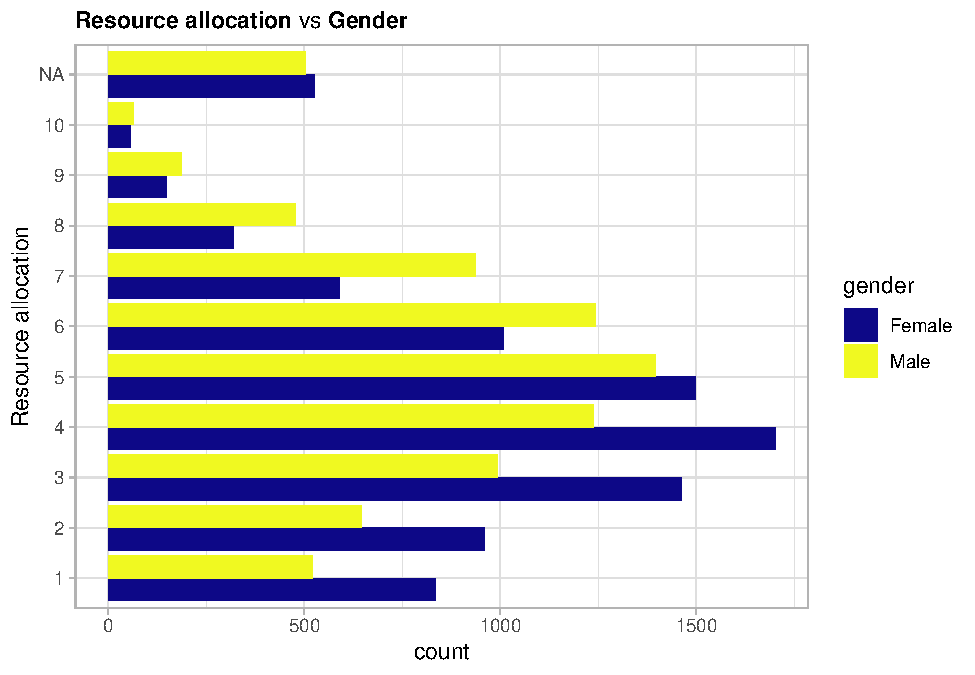
\includegraphics{boosting_methods_files/figure-latex/unnamed-chunk-28-1.pdf}

Here a major shift in distribution is visible towards men getting more resources allocated to them. This reflects the society that still promotes men much more often to high paying jobs that most often come with resource responsibility.

\textbf{Now the mental fatigue score:}

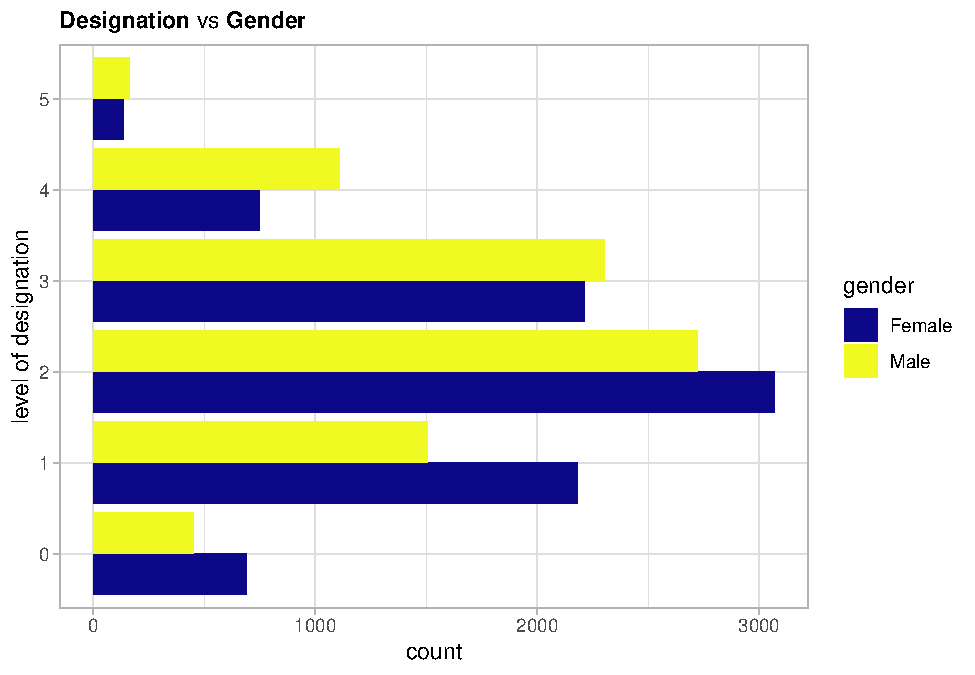
\includegraphics{boosting_methods_files/figure-latex/unnamed-chunk-29-1.pdf}

This is of course very similar to the main effect of the \texttt{gender} variable as the outcome and the feature \texttt{mental\_fatigue\_score} are highly linearly correlated.

\hypertarget{company-type-vs.-the-remaining}{%
\subsubsection{Company type vs.~the remaining}\label{company-type-vs.-the-remaining}}

\begin{Shaded}
\begin{Highlighting}[]
\CommentTok{\# Company type vs Work from home setup}
\FunctionTok{table}\NormalTok{(burnout\_train}\SpecialCharTok{$}\NormalTok{company\_type, burnout\_train}\SpecialCharTok{$}\NormalTok{wfh\_setup\_available)}
\end{Highlighting}
\end{Shaded}

\begin{verbatim}
##          
##             No  Yes
##   Product 2764 3254
##   Service 5165 6118
\end{verbatim}

No notable trend.

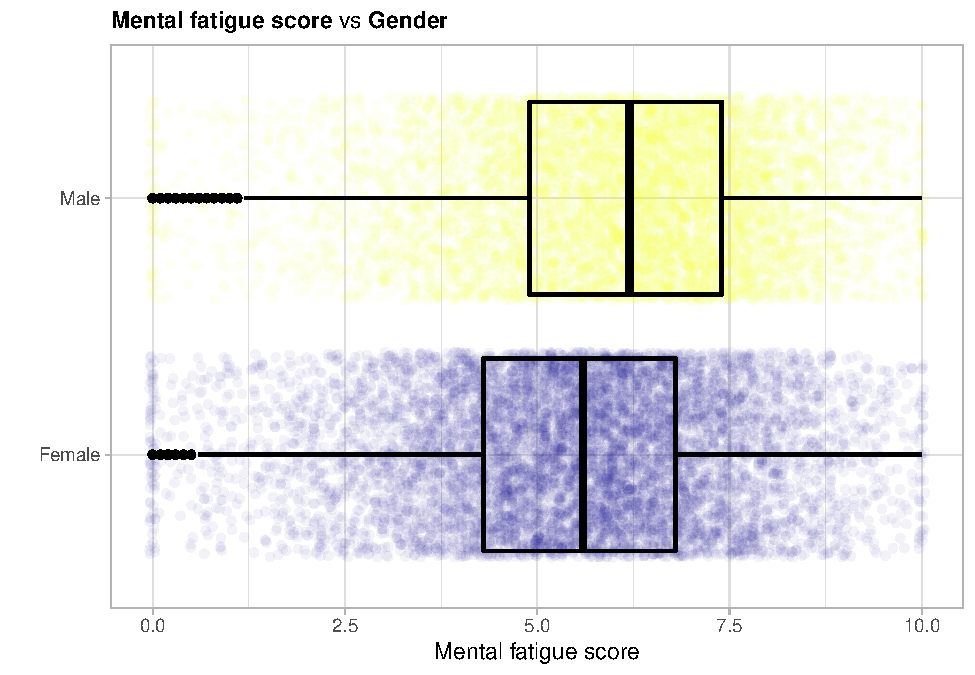
\includegraphics{boosting_methods_files/figure-latex/unnamed-chunk-31-1.pdf}

No trend here either.

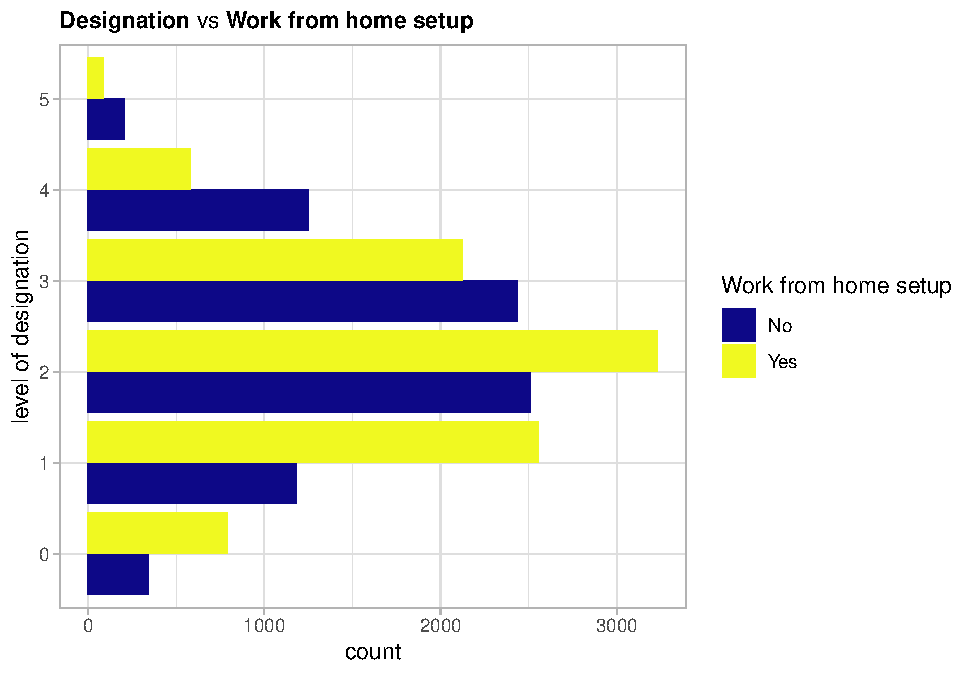
\includegraphics{boosting_methods_files/figure-latex/unnamed-chunk-32-1.pdf}

The same verdict as above.

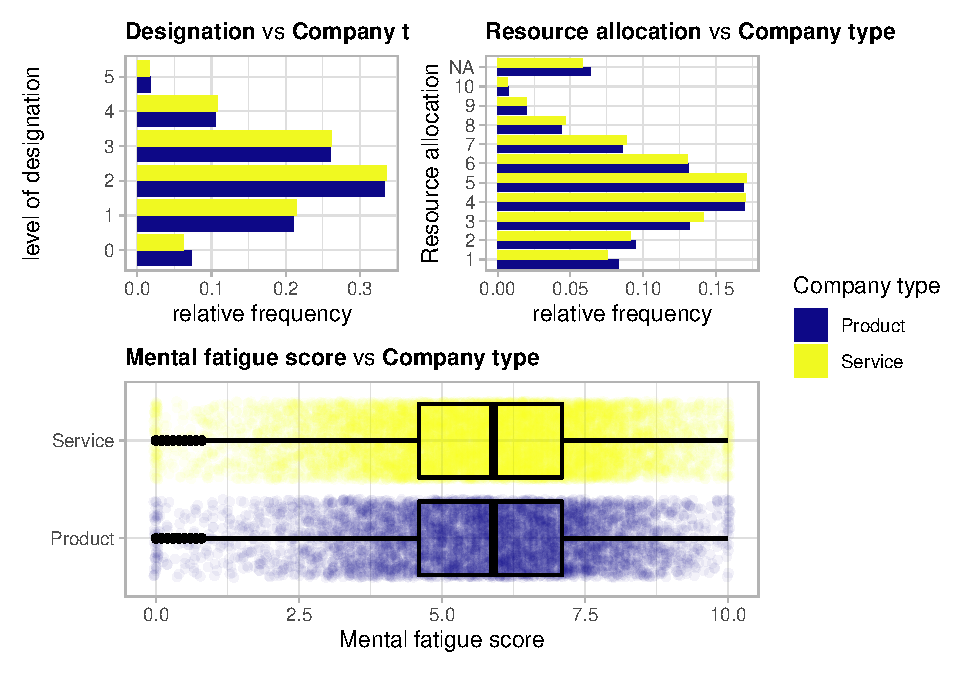
\includegraphics{boosting_methods_files/figure-latex/unnamed-chunk-33-1.pdf}

Once again there is no notable difference in distribution.

\hypertarget{work-from-home-setup-vs.-the-remaining}{%
\subsubsection{Work from home setup vs.~the remaining}\label{work-from-home-setup-vs.-the-remaining}}

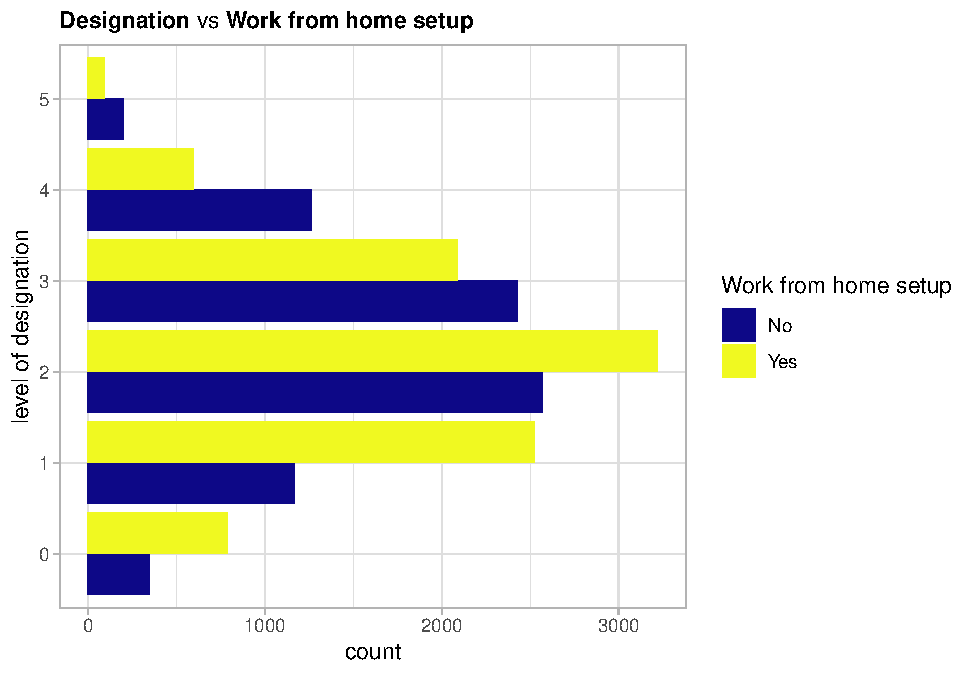
\includegraphics{boosting_methods_files/figure-latex/unnamed-chunk-34-1.pdf}

A work from home setup is way more often available for employees with a lower designation (\(\leq 2\)).

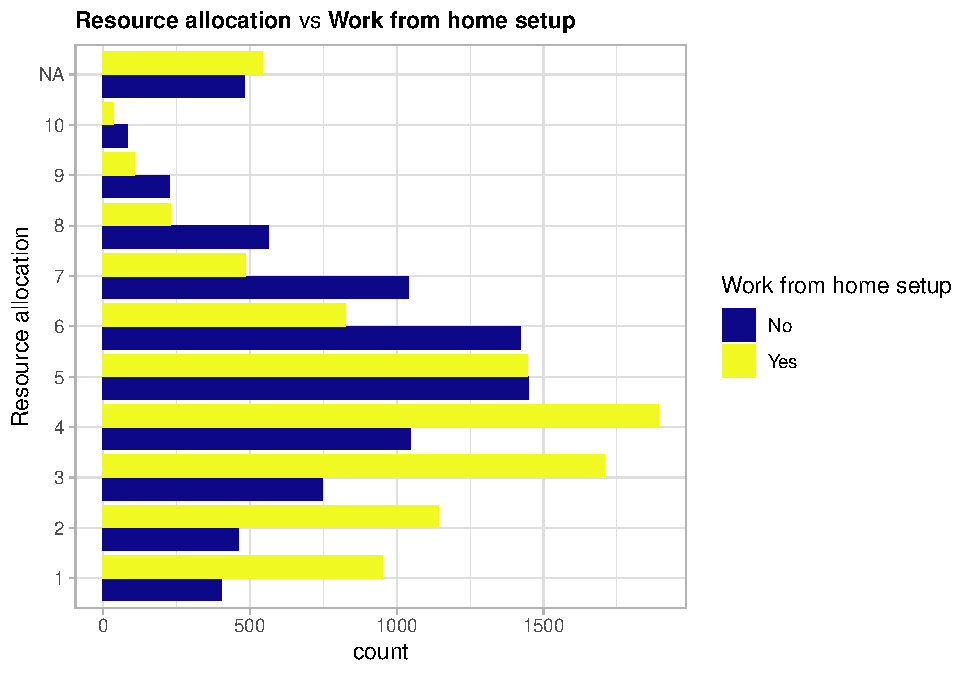
\includegraphics{boosting_methods_files/figure-latex/unnamed-chunk-35-1.pdf}

The same structure as in the previous comparison is visible here again. Employees with a lower amount of resources allocated to them have more often a work from home setup available. This could be due to the fewer responsibilities they have in the business.

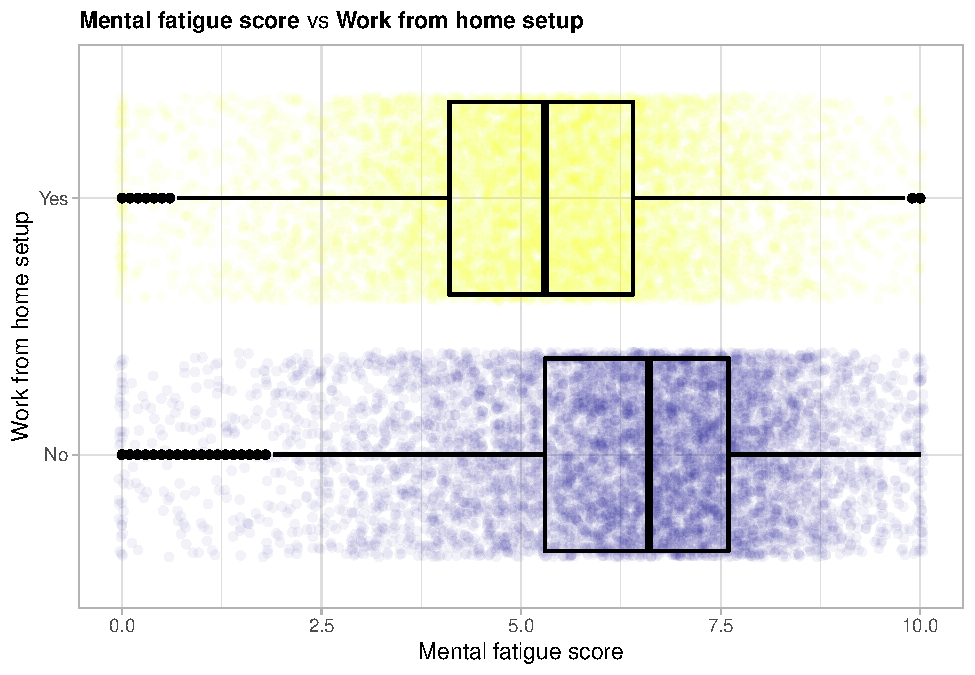
\includegraphics{boosting_methods_files/figure-latex/unnamed-chunk-36-1.pdf}

Again this is of course very similar to the main effect of the \texttt{wfh\_setup\_available} variable as the outcome and the feature \texttt{mental\_fatigue\_score} are highly linearly correlated.

\hypertarget{designation-vs-the-remaining}{%
\subsubsection{Designation vs the remaining}\label{designation-vs-the-remaining}}

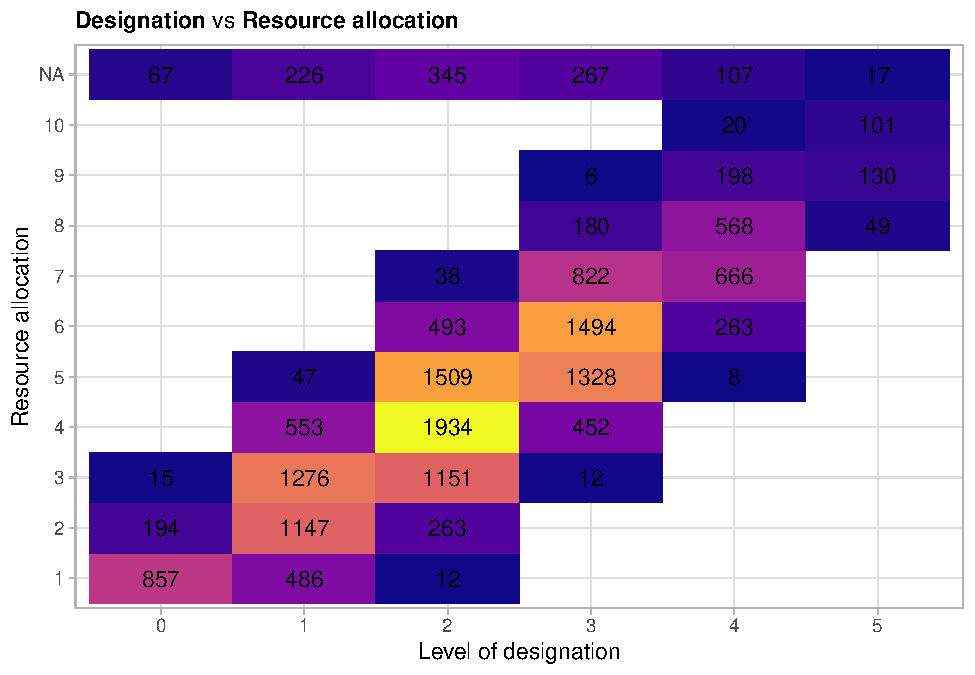
\includegraphics{boosting_methods_files/figure-latex/unnamed-chunk-37-1.pdf}

Here a strong quite linear relationship is visible. This is sensible as often more resource responsibility is given to employees with high designation.

The last two relationships will be omitted here as both for the variable \texttt{designation} as well as for \texttt{resource\_allocation} the comparison with \texttt{mental\_fatigue\_score} will be very similar to the main effect of the two variables. This comes again from the high correlation of the latter with the outcome.

Overall some stronger and mainly less strong relationships between the predictors could be detected. Not like in ordinary least squares regression for gradient tree boosting no decorrelation and normalization of the features is needed.

\hypertarget{some-feature-engineering}{%
\subsection{Some feature engineering}\label{some-feature-engineering}}

The only variable that allows for some reasonable feature engineering is the date of joining predictor. One can try to extract some underlying patterns and see if an effect on the outcome is visible.

First extract the day of the week:

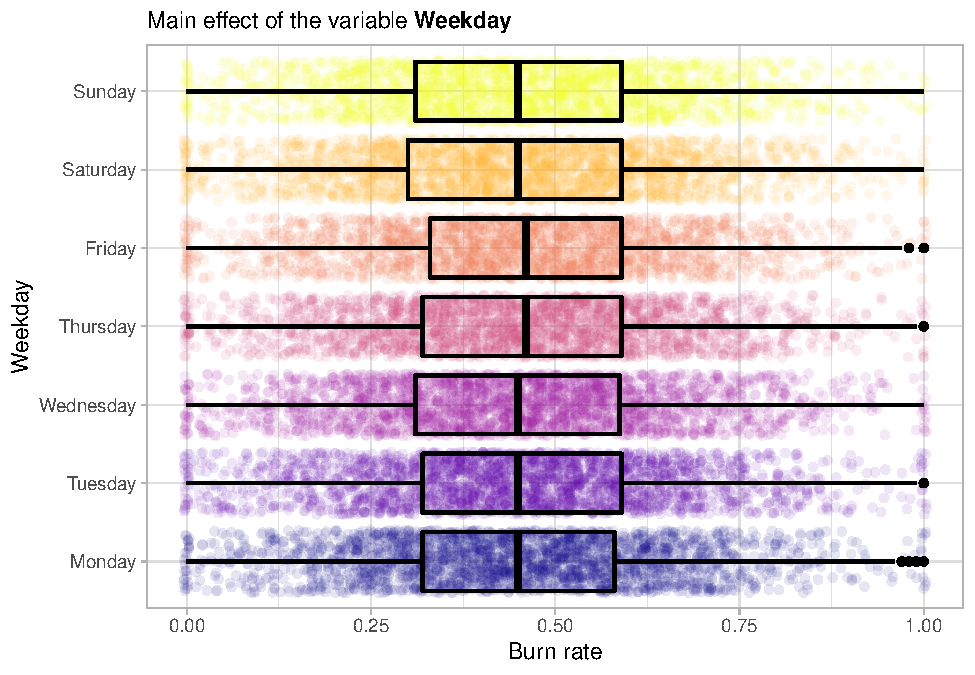
\includegraphics{boosting_methods_files/figure-latex/unnamed-chunk-38-1.pdf}

No main effect is visible here. So try the month next.

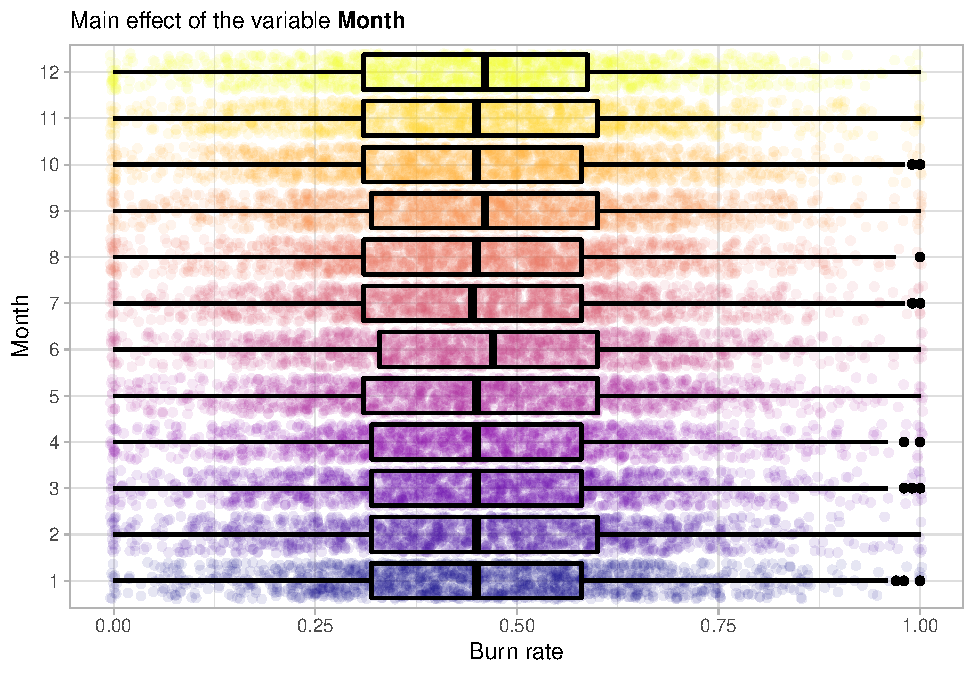
\includegraphics{boosting_methods_files/figure-latex/unnamed-chunk-39-1.pdf}

Again no main effect is visible.

Nevertheless one can include those two variables into the model because as mentioned before tree-based models actually perform a feature selection at each split. So including these just comes only at a small computational cost. This minimal pre-processing that is needed when dealing with tree-based models is actually one of its biggest strengths. It is very robust against any kind of weird selection of features. This is one of the reasons beside the strong predictive power for the heavy use of such models in data mining applications.\citep{elements}

\hypertarget{create-the-recipe}{%
\subsection{Create the recipe}\label{create-the-recipe}}

A recipe is an object that defines a series of steps for data pre-processing and feature engineering.

\begin{Shaded}
\begin{Highlighting}[]
\DocumentationTok{\#\#\# recipe for xgboost (nominal variables must be dummy variables)}
\CommentTok{\# define outcome, predictors and training data set}
\NormalTok{burnout\_rec\_boost }\OtherTok{\textless{}{-}} \FunctionTok{recipe}\NormalTok{(burn\_rate }\SpecialCharTok{\textasciitilde{}}\NormalTok{ date\_of\_joining }\SpecialCharTok{+}\NormalTok{ gender }\SpecialCharTok{+}
\NormalTok{                            company\_type }\SpecialCharTok{+}\NormalTok{ wfh\_setup\_available }\SpecialCharTok{+}
\NormalTok{                            designation }\SpecialCharTok{+}\NormalTok{ resource\_allocation }\SpecialCharTok{+}
\NormalTok{                            mental\_fatigue\_score,}
                            \AttributeTok{data =}\NormalTok{ burnout\_train) }\SpecialCharTok{\%\textgreater{}\%}
  \CommentTok{\# extract the date features day of the week and month}
  \FunctionTok{step\_date}\NormalTok{(date\_of\_joining, }\AttributeTok{features =} \FunctionTok{c}\NormalTok{(}\StringTok{"dow"}\NormalTok{, }\StringTok{"month"}\NormalTok{)) }\SpecialCharTok{\%\textgreater{}\%}
  \CommentTok{\# dummify all nominal features}
  \FunctionTok{step\_dummy}\NormalTok{(}\FunctionTok{all\_nominal}\NormalTok{()) }\SpecialCharTok{\%\textgreater{}\%}
  \CommentTok{\# encode the date as integers}
  \FunctionTok{step\_mutate}\NormalTok{(}\AttributeTok{date\_of\_joining =} \FunctionTok{as.integer}\NormalTok{(date\_of\_joining))}

\DocumentationTok{\#\#\# recipe for a random forest model for comparison (no dummy encoding needed)}
\CommentTok{\# same as above without dummification}
\NormalTok{burnout\_rec\_rf }\OtherTok{\textless{}{-}} \FunctionTok{recipe}\NormalTok{(burn\_rate }\SpecialCharTok{\textasciitilde{}}\NormalTok{ date\_of\_joining }\SpecialCharTok{+}\NormalTok{ gender }\SpecialCharTok{+}
\NormalTok{                         company\_type }\SpecialCharTok{+}\NormalTok{ wfh\_setup\_available }\SpecialCharTok{+}
\NormalTok{                         designation }\SpecialCharTok{+}\NormalTok{ resource\_allocation }\SpecialCharTok{+}
\NormalTok{                         mental\_fatigue\_score,}
                         \AttributeTok{data =}\NormalTok{ burnout\_train) }\SpecialCharTok{\%\textgreater{}\%}
  \FunctionTok{step\_date}\NormalTok{(date\_of\_joining, }\AttributeTok{features =} \FunctionTok{c}\NormalTok{(}\StringTok{"dow"}\NormalTok{, }\StringTok{"month"}\NormalTok{)) }\SpecialCharTok{\%\textgreater{}\%}
  \FunctionTok{step\_mutate}\NormalTok{(}\AttributeTok{date\_of\_joining =} \FunctionTok{as.integer}\NormalTok{(date\_of\_joining))}
\end{Highlighting}
\end{Shaded}

\hypertarget{insurence-data}{%
\section{Insurence data}\label{insurence-data}}

The insurance data set is part of the book \emph{Machine Learning with R} by Brett Lantz. It can be downloaded here:
\url{https://raw.githubusercontent.com/stedy/Machine-Learning-with-R-datasets/master/insurance.csv}

\begin{Shaded}
\begin{Highlighting}[]
\CommentTok{\# load the data}
\NormalTok{insurance\_data }\OtherTok{\textless{}{-}} \FunctionTok{read\_csv}\NormalTok{(}\StringTok{"\_data/insurance.csv"}\NormalTok{)}
\end{Highlighting}
\end{Shaded}

\hypertarget{train-test-split-1}{%
\subsection{Train-test split}\label{train-test-split-1}}

\begin{Shaded}
\begin{Highlighting}[]
\FunctionTok{set.seed}\NormalTok{(}\DecValTok{2}\NormalTok{)}
\NormalTok{ins\_split }\OtherTok{\textless{}{-}}\NormalTok{ rsample}\SpecialCharTok{::}\FunctionTok{initial\_split}\NormalTok{(insurance\_data, }\AttributeTok{prop =} \FloatTok{0.80}\NormalTok{)}
\NormalTok{ins\_train }\OtherTok{\textless{}{-}}\NormalTok{ rsample}\SpecialCharTok{::}\FunctionTok{training}\NormalTok{(ins\_split)}
\NormalTok{ins\_test  }\OtherTok{\textless{}{-}}\NormalTok{ rsample}\SpecialCharTok{::}\FunctionTok{testing}\NormalTok{(ins\_split)}
\end{Highlighting}
\end{Shaded}

\hypertarget{a-general-overview}{%
\subsection{A general overview}\label{a-general-overview}}

A general visualization to detect missing values.

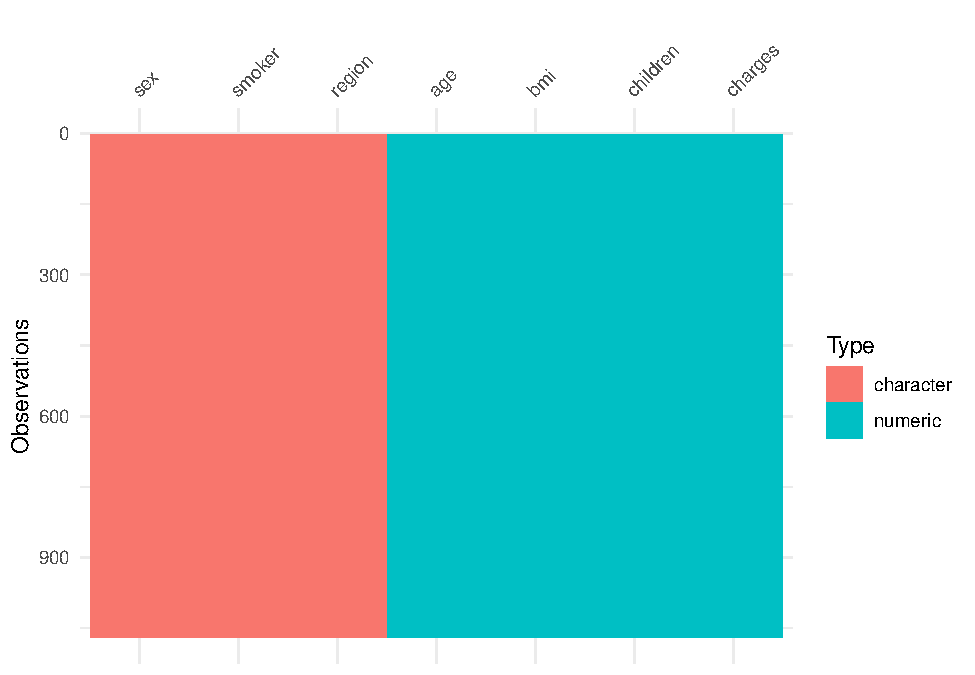
\includegraphics{boosting_methods_files/figure-latex/visdatIns-1.pdf}
So there are no missing values!

\hypertarget{what-about-the-outcome}{%
\subsection{What about the outcome?}\label{what-about-the-outcome}}

\texttt{charges}: Individual medical costs billed by health insurance.

The five point summary below shows that the no invalid values i.e.~negative ones are in the data.

\begin{verbatim}
##    Min. 1st Qu.  Median    Mean 3rd Qu.    Max. 
##    1122    4703    9433   13128   16436   63770
\end{verbatim}

Now the distribution of the outcome.

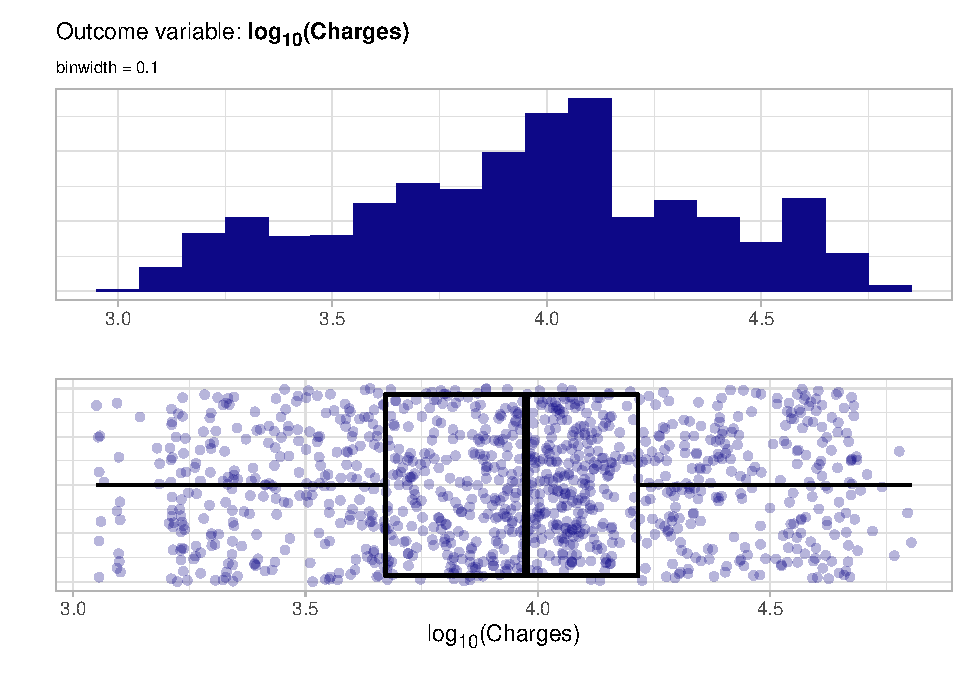
\includegraphics{boosting_methods_files/figure-latex/unnamed-chunk-42-1.pdf}
Not like the \texttt{burn\_rate} previously this target distribution is not at all symmetrical but highly right skewed. A natural thing to do would be a log transformation of the outcome. The resulting \texttt{log\_charges} outcome variable is shown below.

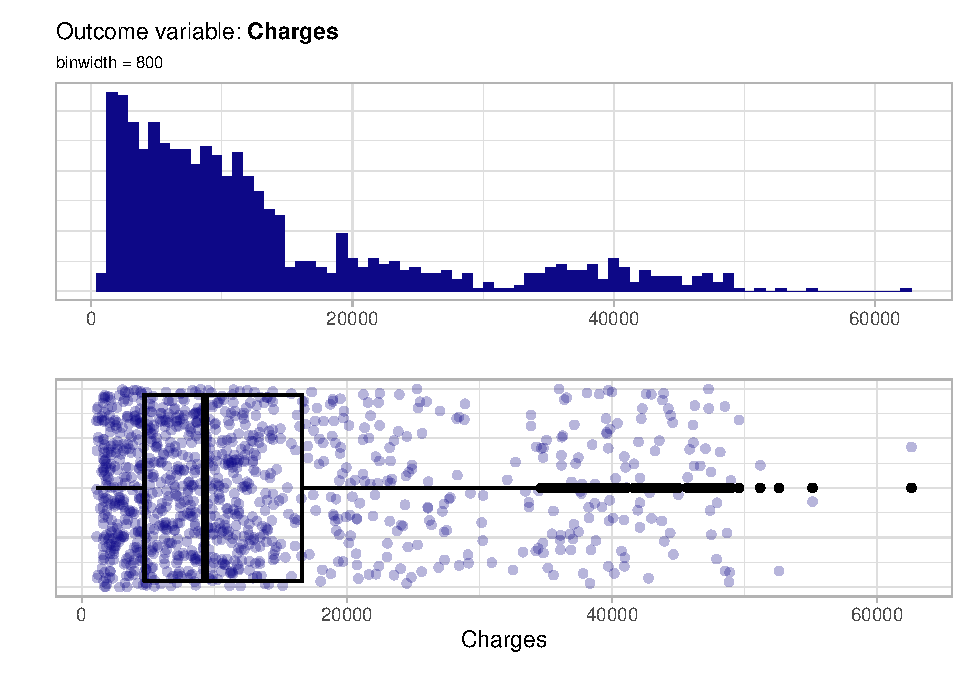
\includegraphics{boosting_methods_files/figure-latex/unnamed-chunk-43-1.pdf}

Although such a transformation of the outcome variable is not needed for tree-based modeling it can make the job of the algorithm somewhat easier.

\hypertarget{distribution-and-main-effects-of-the-predictors-1}{%
\subsection{Distribution and main effects of the predictors}\label{distribution-and-main-effects-of-the-predictors-1}}

\hypertarget{age}{%
\subsubsection{Age}\label{age}}

\texttt{age}: The age of the insurance contractor. This is naturally a continuous variable.

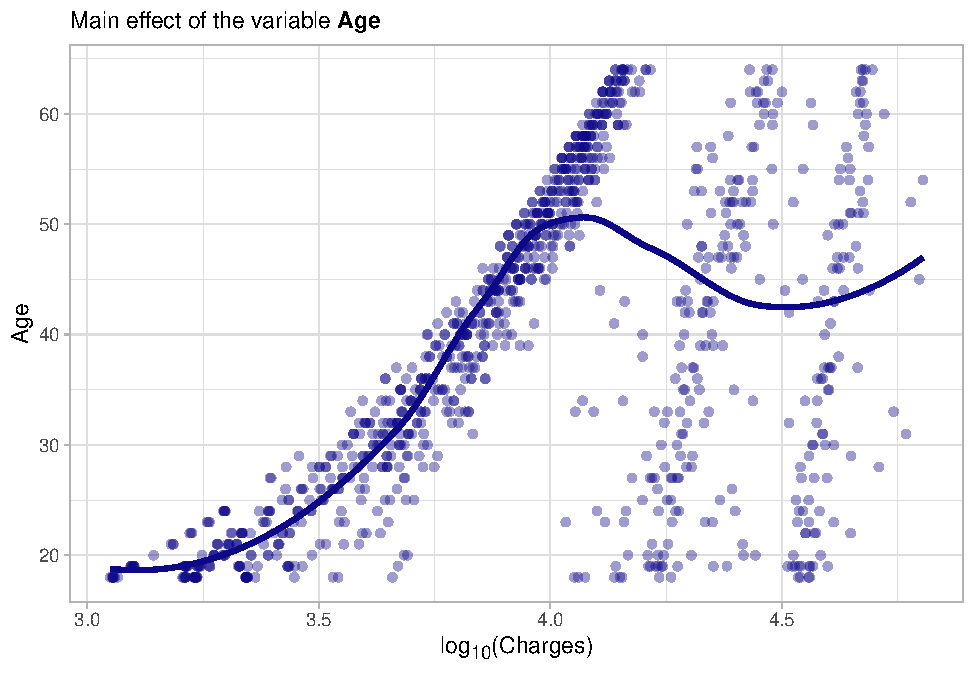
\includegraphics{boosting_methods_files/figure-latex/unnamed-chunk-44-1.pdf}

A wide range of ages is covered. Notably there is a peak at roughly 18 which means that many fresh adults were observed in this data set.

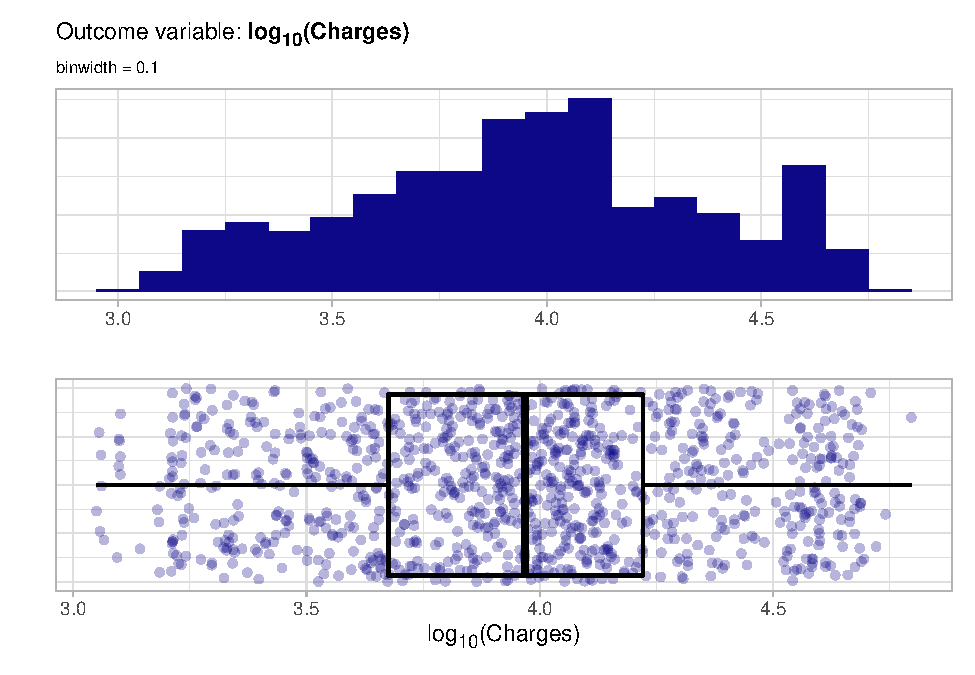
\includegraphics{boosting_methods_files/figure-latex/unnamed-chunk-45-1.pdf}

There seems to be a strong main effect although it does not seem to be linear. The general trend is that older contractors generally accumulate more medical costs. This is very intuitive.

\hypertarget{sex}{%
\subsubsection{Sex}\label{sex}}

\texttt{sex}: The insurance contractors gender. Here either female or male. This means it is a binary variable and will be treated as such.

\begin{Shaded}
\begin{Highlighting}[]
\FunctionTok{summary}\NormalTok{(}\FunctionTok{as.factor}\NormalTok{(ins\_train}\SpecialCharTok{$}\NormalTok{sex))}
\end{Highlighting}
\end{Shaded}

\begin{verbatim}
## female   male 
##    534    537
\end{verbatim}

The classes are very well balanced. Now the main effect.

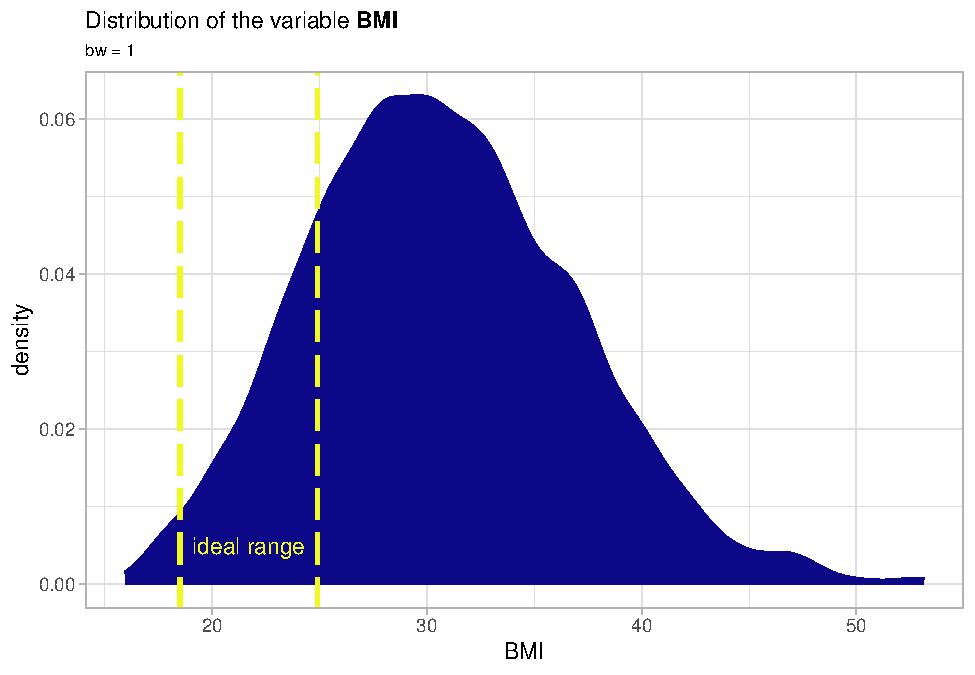
\includegraphics{boosting_methods_files/figure-latex/unnamed-chunk-47-1.pdf}

No notable difference can be detected here.

\hypertarget{body-mass-index}{%
\subsubsection{Body mass index}\label{body-mass-index}}

\texttt{bmi}: The body mass index is providing an understanding of the body composition. It is a ratio composed out of the weight which is divided by the height \(\frac{kg}{m^2}\). Ideally the ratio is between 18.5 and 24.9. The variable is obviously a continuous variable.

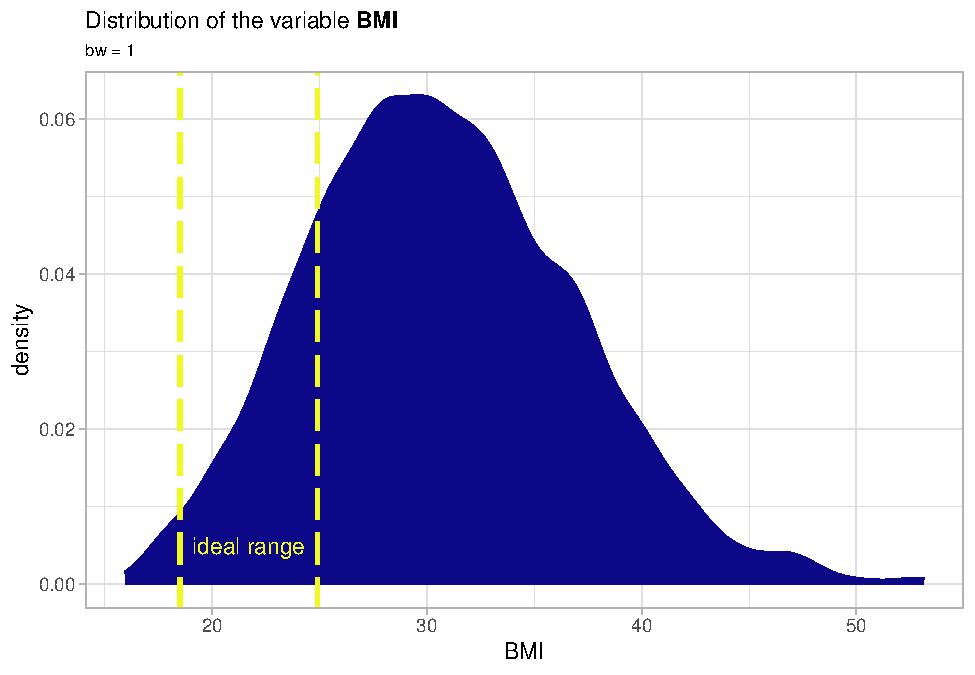
\includegraphics{boosting_methods_files/figure-latex/unnamed-chunk-48-1.pdf}

The distribution is bell-shaped and symmetrical roughly around a bmi of 30 which is above the ideal range. Actually only a small amount of the data falls into the normal range here. Moreover the right tail is heavier than the left one. Now a look at the main effect of the variable.

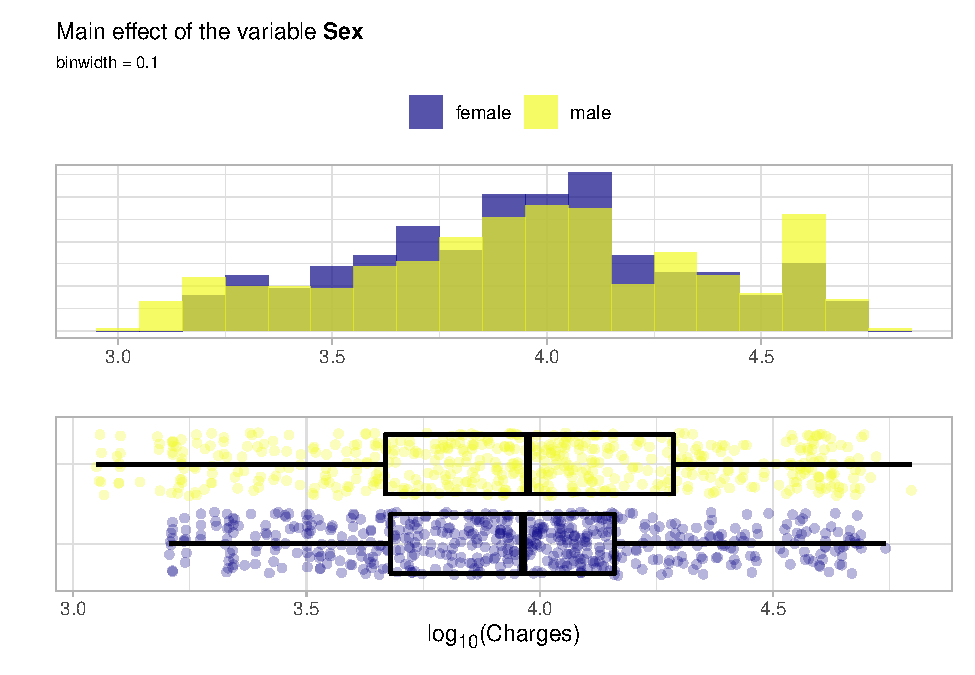
\includegraphics{boosting_methods_files/figure-latex/unnamed-chunk-49-1.pdf}

With some fantasy one can grasp some non-linear patterns on the right side of the plot but beside that no strong main effect is visible here.

\hypertarget{number-of-children}{%
\subsubsection{Number of children}\label{number-of-children}}

\texttt{children}: The number of children or dependents covered by the health insurance.

\begin{Shaded}
\begin{Highlighting}[]
\CommentTok{\# unique values of the feature}
\FunctionTok{unique}\NormalTok{(ins\_train}\SpecialCharTok{$}\NormalTok{children)}
\end{Highlighting}
\end{Shaded}

\begin{verbatim}
## [1] 0 1 3 2 5 4
\end{verbatim}

This could be treated as categorical but as there is a natural ordering it will be encoded by the integers so the treatment is like the one of a continuous feature.

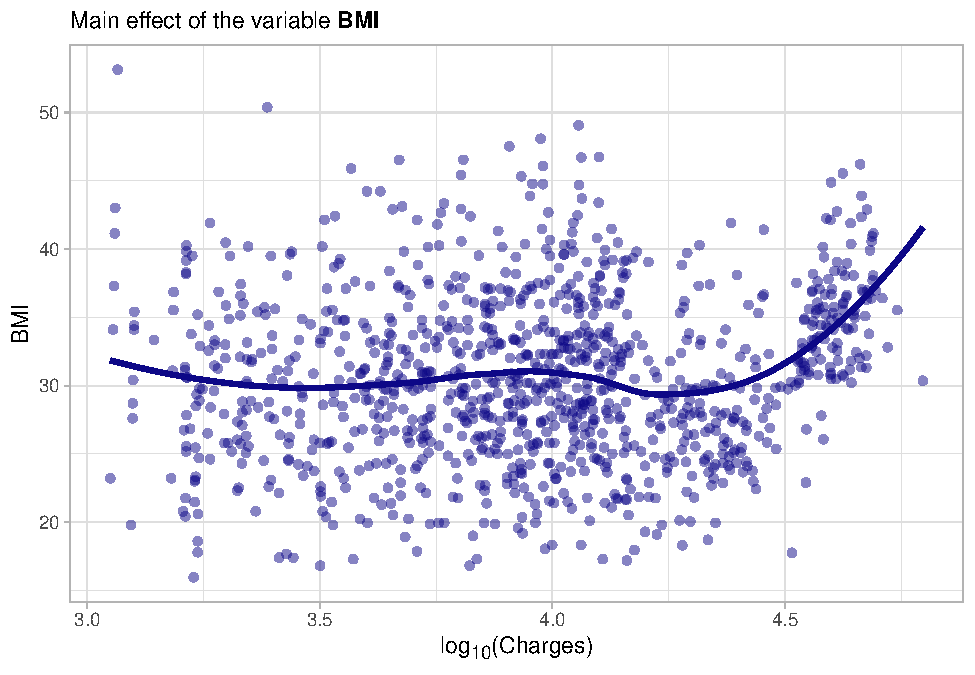
\includegraphics{boosting_methods_files/figure-latex/unnamed-chunk-51-1.pdf}

As one would also think the more children the lower the number of observed values. Especially the numbers greater than 3 are not well represented. If encoded by one-hot-encoding one would have to think about removing these then near-zero-variance variables. But as they will be encoded in a continuous way this is no problem at all. A look at the main effects can now strengthen or weaken this hypothesis of a natural ordering.

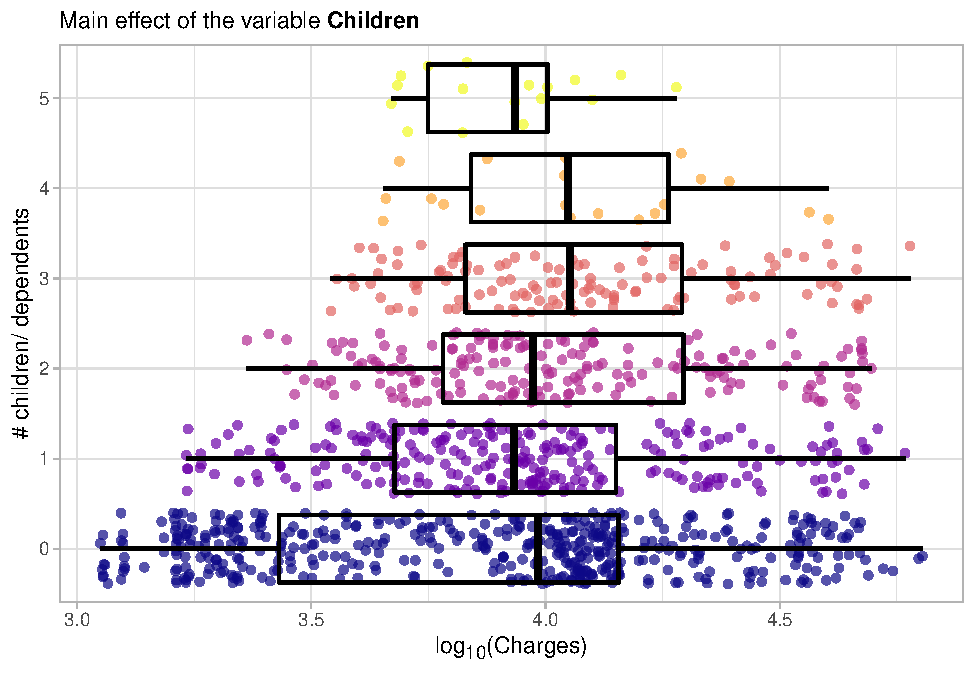
\includegraphics{boosting_methods_files/figure-latex/unnamed-chunk-52-1.pdf}

This plot is quite similar to the main effect plot for the \texttt{age} feature. As most likely (will be checked later) the age is positively correlated with the number of children one can observe a rise of the minimal observed charges towards a greater amount of children. The upper two boxplots are built with just a few observations so they should not be interpreted in great detail. Overall there seems to be some kind of main effect.

\hypertarget{smoking}{%
\subsubsection{Smoking}\label{smoking}}

\texttt{smoker}: Is the contractor smoking? Of course a binary variable.

\begin{Shaded}
\begin{Highlighting}[]
\FunctionTok{summary}\NormalTok{(}\FunctionTok{as.factor}\NormalTok{(ins\_train}\SpecialCharTok{$}\NormalTok{smoker))}
\end{Highlighting}
\end{Shaded}

\begin{verbatim}
##  no yes 
## 859 212
\end{verbatim}

The classes are not balanced but the class of the smokers is still represented with a good amount of observations. Now a look at the main effect.

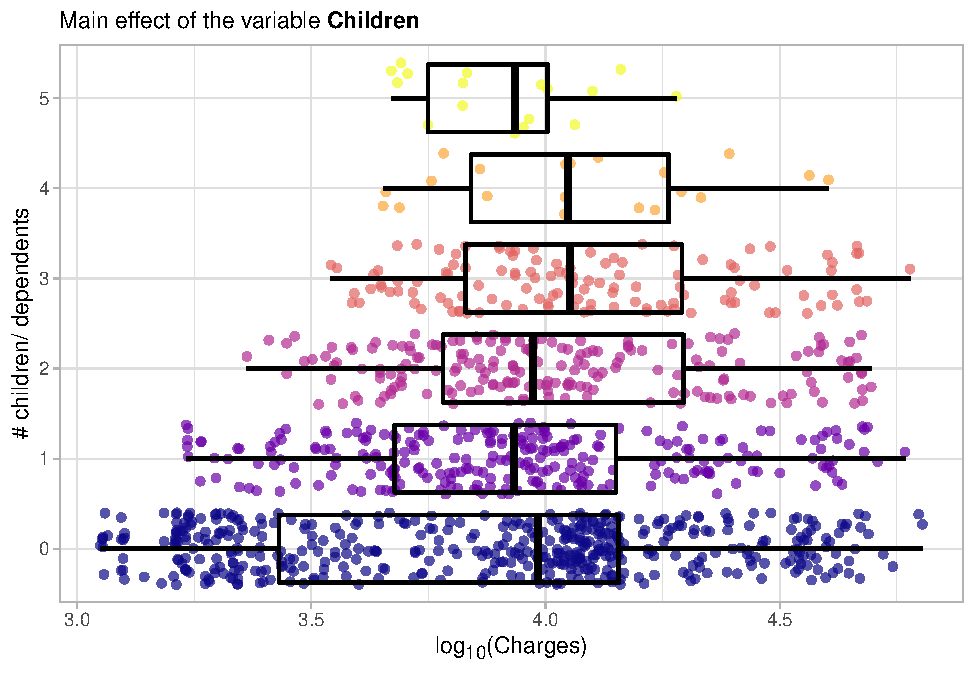
\includegraphics{boosting_methods_files/figure-latex/unnamed-chunk-54-1.pdf}

This main effect is as drastic as it is intuitive. Smoking seems to definitely increases the charges. This means that this variable has probably a lot of predictive power.

\hypertarget{region}{%
\subsubsection{Region}\label{region}}

\texttt{region}: The beneficiary's residential area in the US. Either northeast, southeast, southwest or northwest. This definitely is a categorical variable.

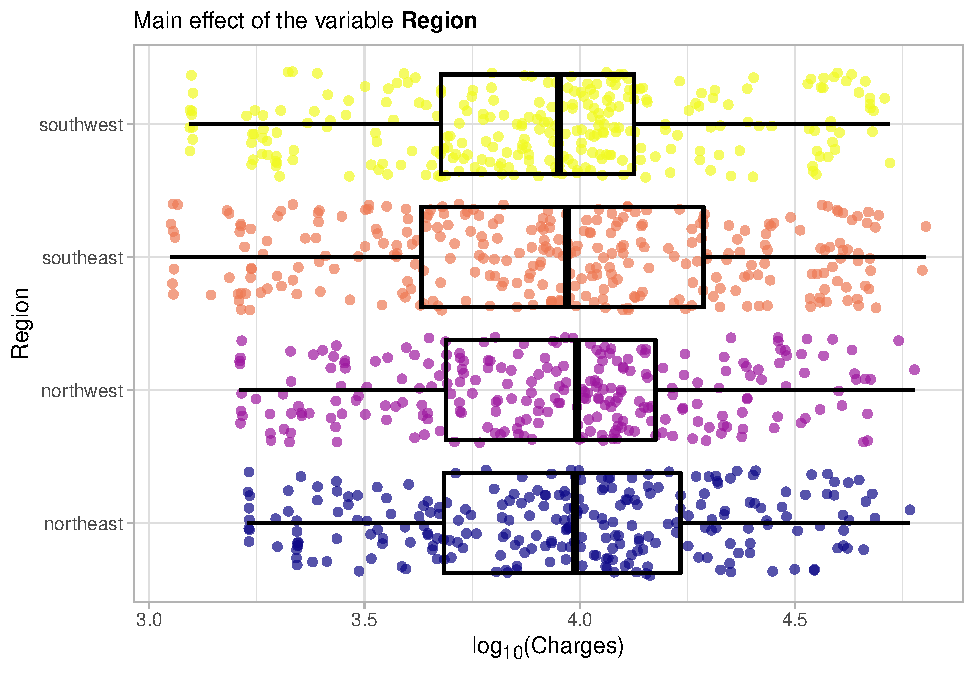
\includegraphics{boosting_methods_files/figure-latex/unnamed-chunk-55-1.pdf}

The four regions are balanced. Now to the main effect.

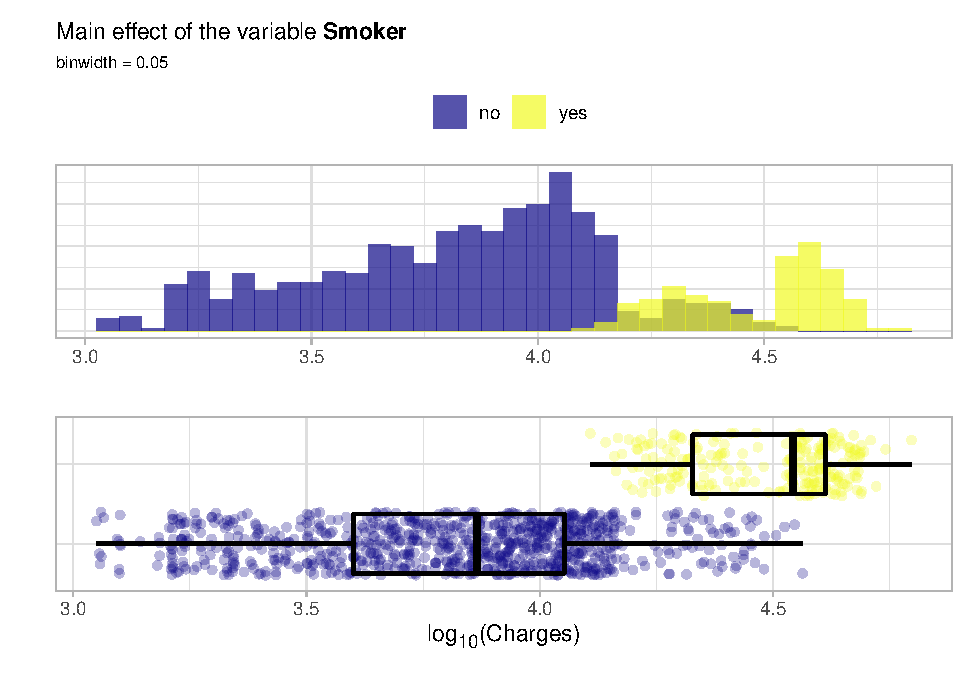
\includegraphics{boosting_methods_files/figure-latex/unnamed-chunk-56-1.pdf}

No important main effect is detectable from this plot.

\hypertarget{relationships-between-the-predictors-1}{%
\subsection{Relationships between the predictors}\label{relationships-between-the-predictors-1}}

\hypertarget{age-vs-the-others}{%
\subsubsection{Age vs the others}\label{age-vs-the-others}}

First the continuous one: \texttt{bmi}

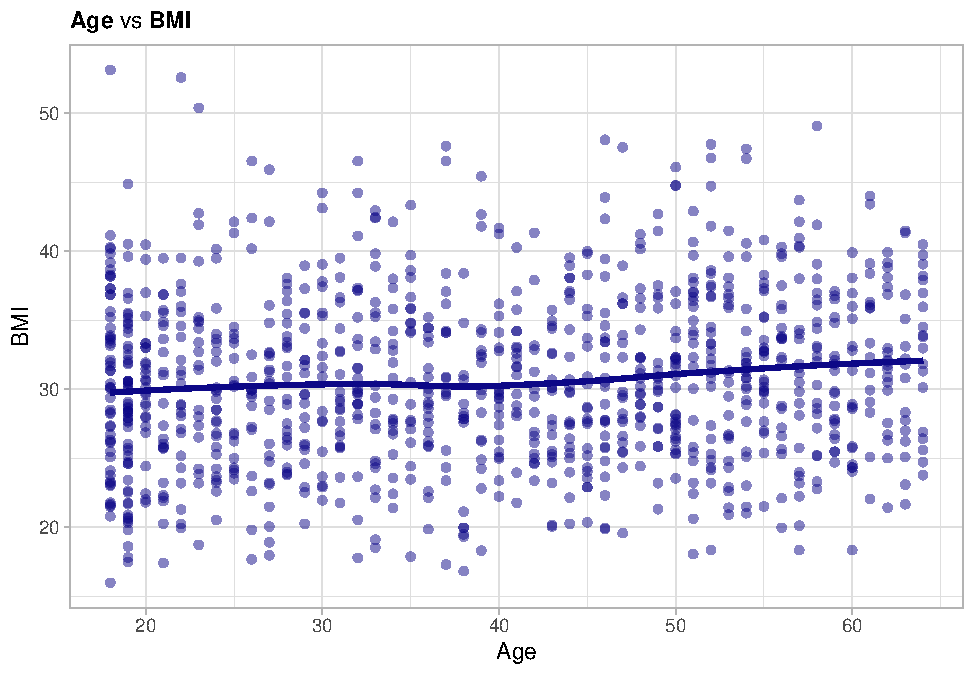
\includegraphics{boosting_methods_files/figure-latex/unnamed-chunk-57-1.pdf}

No relationship detectable. The pearson correlation is with 0.109 also low.

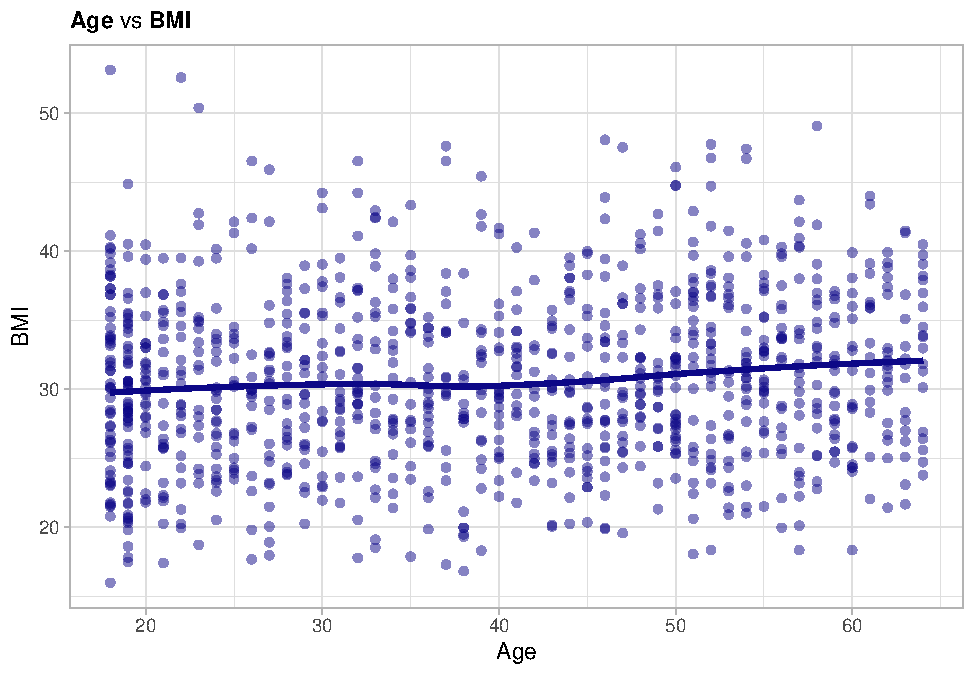
\includegraphics{boosting_methods_files/figure-latex/unnamed-chunk-59-1.pdf}

The most interesting take away from these four plots is that the hypothesis about the age of the contractors with children seem to be okish except for the ones with more than 3 children. But again this counterintuitive behavior could also be due to the few samples. At this point one might think about encoding the children variable as a categorical but in the following it will be left continuous.

\hypertarget{sex-vs-the-remaining}{%
\subsubsection{Sex vs the remaining}\label{sex-vs-the-remaining}}

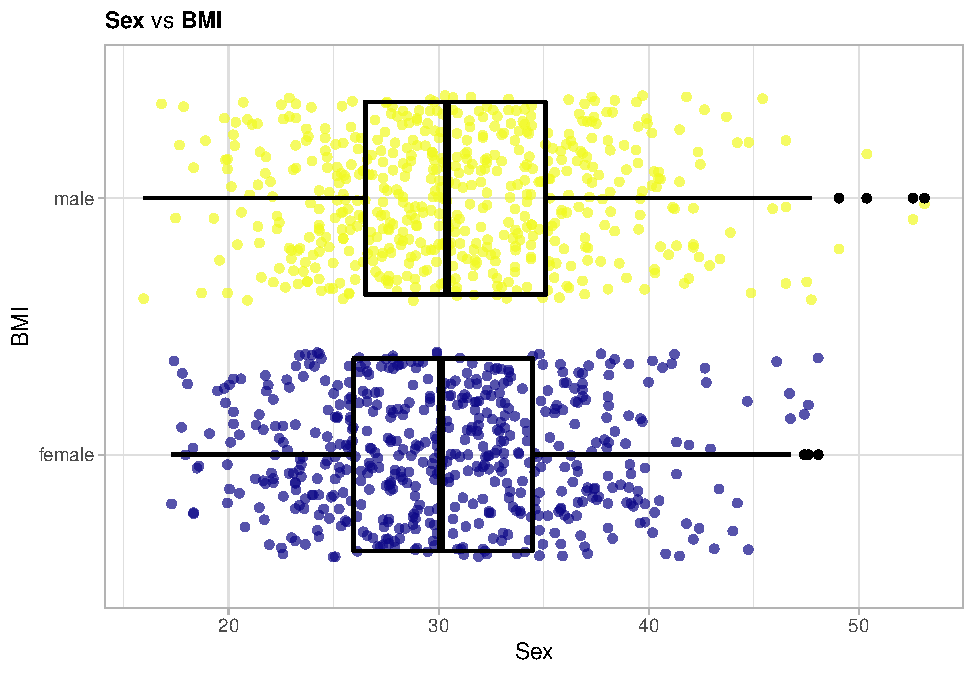
\includegraphics{boosting_methods_files/figure-latex/unnamed-chunk-60-1.pdf}

Not a huge difference.

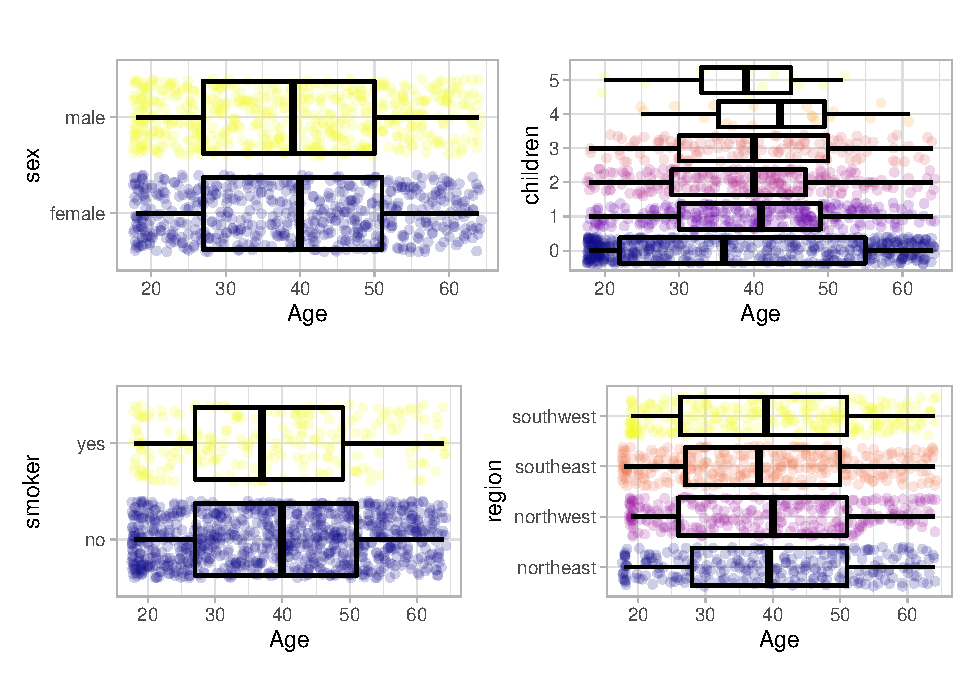
\includegraphics{boosting_methods_files/figure-latex/unnamed-chunk-61-1.pdf}

Also quite balanced.

Contingency table for the binary variable \texttt{smoker}:

\begin{Shaded}
\begin{Highlighting}[]
\CommentTok{\# sex vs smoker}
\FunctionTok{table}\NormalTok{(ins\_train}\SpecialCharTok{$}\NormalTok{sex, ins\_train}\SpecialCharTok{$}\NormalTok{smoker)}
\end{Highlighting}
\end{Shaded}

\begin{verbatim}
##         
##           no yes
##   female 450  84
##   male   409 128
\end{verbatim}

Slightly more men smoke but the difference is smallish.

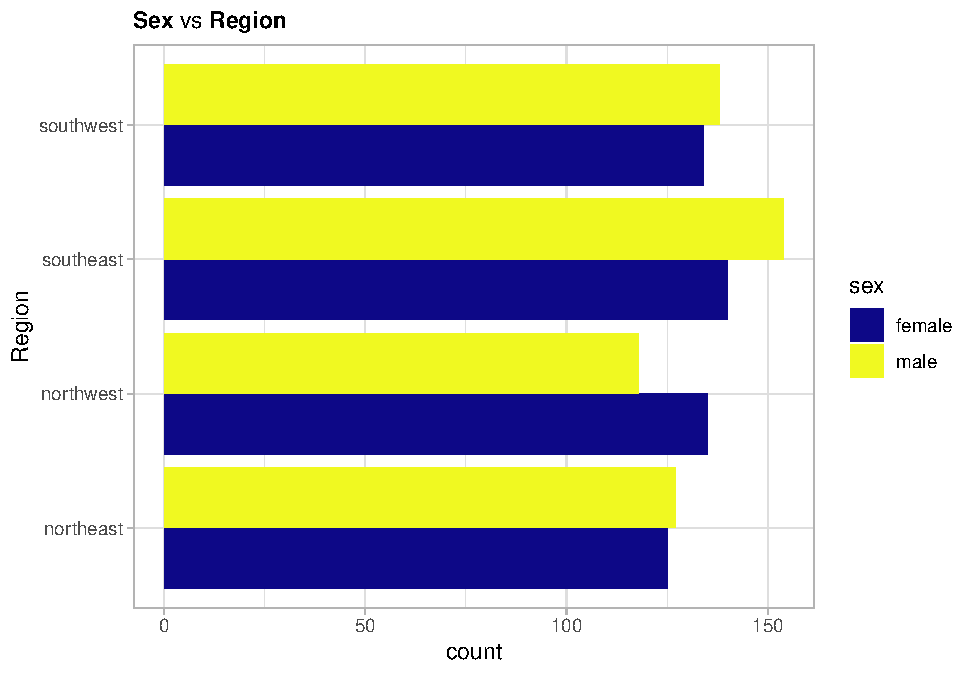
\includegraphics{boosting_methods_files/figure-latex/unnamed-chunk-63-1.pdf}

No notable differences.

\hypertarget{bmi-vs-the-remaining}{%
\subsubsection{BMI vs the remaining}\label{bmi-vs-the-remaining}}

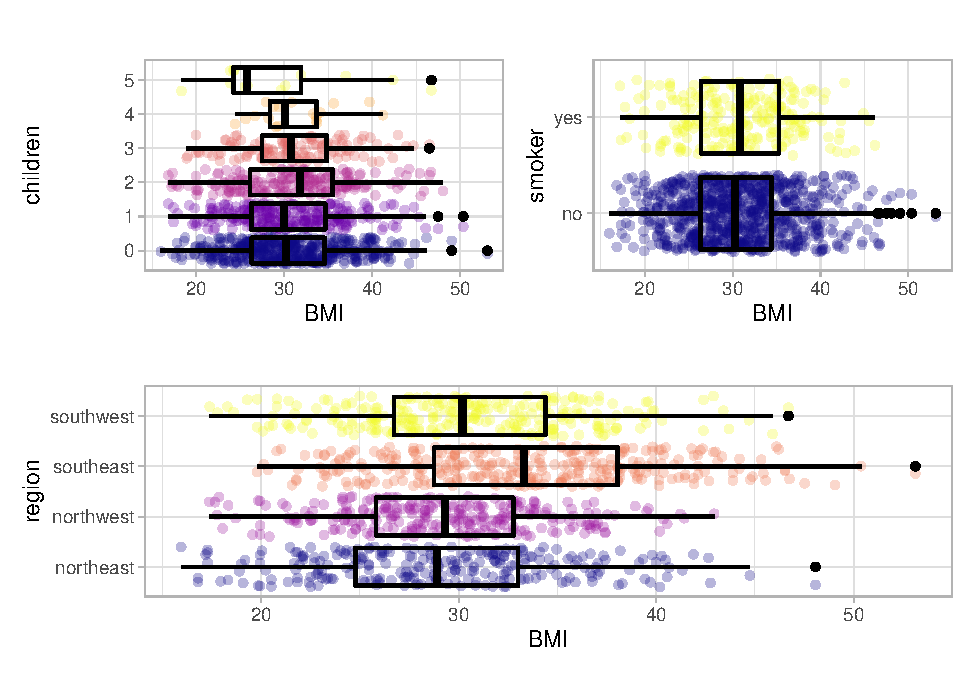
\includegraphics{boosting_methods_files/figure-latex/unnamed-chunk-64-1.pdf}

The most notable fact here is that southeast of the US seems to be a little more overweight than the rest.

\hypertarget{children-vs-the-remaining}{%
\subsubsection{Children vs the remaining}\label{children-vs-the-remaining}}

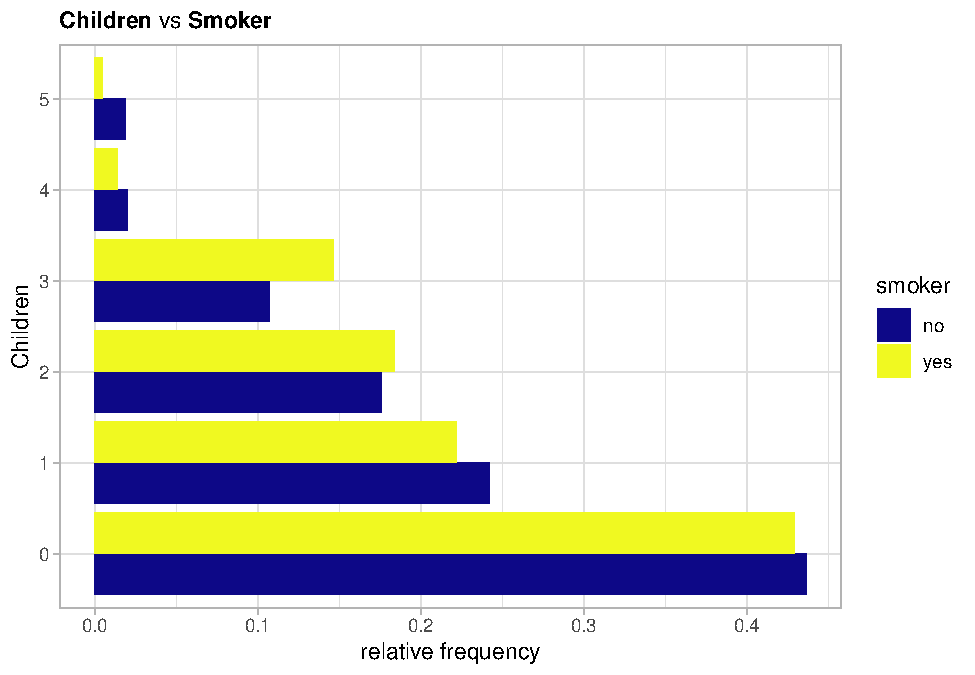
\includegraphics{boosting_methods_files/figure-latex/unnamed-chunk-65-1.pdf}

In relative terms actually the contractors with three children smoke the most but the other levels seem quite balanced.

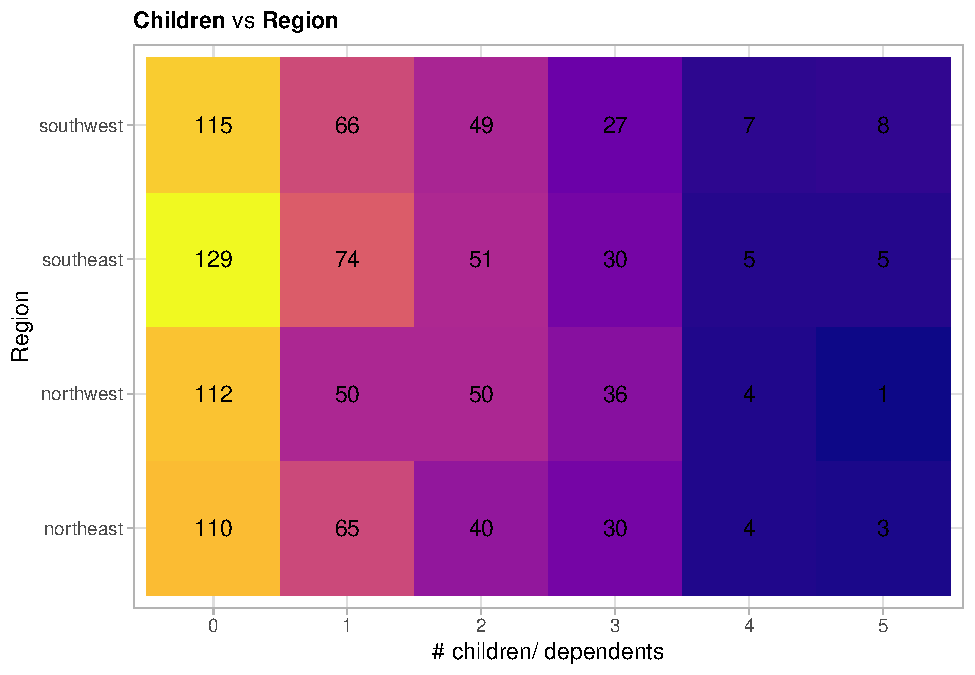
\includegraphics{boosting_methods_files/figure-latex/unnamed-chunk-66-1.pdf}

Here no trend is visible.

\hypertarget{smoker-vs-region}{%
\subsubsection{Smoker vs Region}\label{smoker-vs-region}}

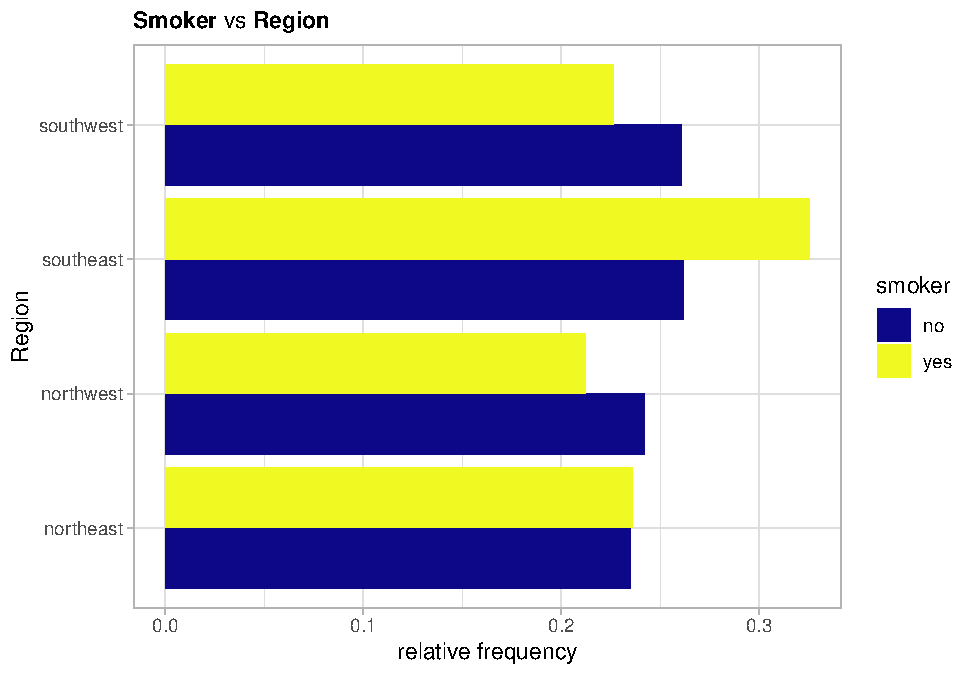
\includegraphics{boosting_methods_files/figure-latex/unnamed-chunk-67-1.pdf}

So the southeast is not only the most overweight region but also the one with the most smokers in relative terms.

This concludes the tour of the pairwise relationships. Besides a crystal clear understanding of the data one sees that there is not much room left for feature engineering. Thus one can go on and define the recipe.

\hypertarget{create-the-recipe-1}{%
\subsection{Create the recipe}\label{create-the-recipe-1}}

Transformations on the outcome variable are not done within a recipe thus this will be done now before hand by adding a new feature i.e.~\texttt{log10\_charges} to the train and test data set.

\begin{Shaded}
\begin{Highlighting}[]
\CommentTok{\# add the log transformed outcome variable to the data}
\NormalTok{ins\_train}\SpecialCharTok{$}\NormalTok{log10\_charges }\OtherTok{\textless{}{-}} \FunctionTok{log10}\NormalTok{(ins\_train}\SpecialCharTok{$}\NormalTok{charges)}
\NormalTok{ins\_test}\SpecialCharTok{$}\NormalTok{log10\_charges }\OtherTok{\textless{}{-}} \FunctionTok{log10}\NormalTok{(ins\_test}\SpecialCharTok{$}\NormalTok{charges)}
\end{Highlighting}
\end{Shaded}

\begin{Shaded}
\begin{Highlighting}[]
\DocumentationTok{\#\#\# recipe for xgboost (nominal variables must be dummy variables)}
\CommentTok{\# define outcome, predictors and training data set}
\NormalTok{burnout\_rec\_boost }\OtherTok{\textless{}{-}} \FunctionTok{recipe}\NormalTok{(log10\_charges }\SpecialCharTok{\textasciitilde{}}\NormalTok{ age }\SpecialCharTok{+}\NormalTok{ sex }\SpecialCharTok{+}
\NormalTok{                            bmi }\SpecialCharTok{+}\NormalTok{ children }\SpecialCharTok{+}
\NormalTok{                            smoker }\SpecialCharTok{+}\NormalTok{ region,}
                            \AttributeTok{data =}\NormalTok{ ins\_train) }\SpecialCharTok{\%\textgreater{}\%}
  \CommentTok{\# dummify all nominal features (sex, smoker, region)}
  \FunctionTok{step\_dummy}\NormalTok{(}\FunctionTok{all\_nominal}\NormalTok{())}

\DocumentationTok{\#\#\# recipe for a random forest model for comparison (no dummy encoding needed)}
\CommentTok{\# same as above without dummification}
\NormalTok{burnout\_rec\_rf }\OtherTok{\textless{}{-}} \FunctionTok{recipe}\NormalTok{(log10\_charges }\SpecialCharTok{\textasciitilde{}}\NormalTok{ age }\SpecialCharTok{+}\NormalTok{ sex }\SpecialCharTok{+}
\NormalTok{                         bmi }\SpecialCharTok{+}\NormalTok{ children }\SpecialCharTok{+}
\NormalTok{                         smoker }\SpecialCharTok{+}\NormalTok{ region,}
                         \AttributeTok{data =}\NormalTok{ ins\_train)}
\end{Highlighting}
\end{Shaded}

Having now all the recipes ready one can proceed with modeling. Finally!

\hypertarget{modeling}{%
\chapter{Let's boost the models}\label{modeling}}

For modeling two additional packages are required.\citep[\citet{ranger_package}]{xgboost_package}

\begin{Shaded}
\begin{Highlighting}[]
\FunctionTok{library}\NormalTok{(xgboost)}
\FunctionTok{library}\NormalTok{(ranger)}
\end{Highlighting}
\end{Shaded}

First one has to set a metric for the evaluation of the final performance. This will be the mean average error (MAE) which is kind of the \(L_1\) norm of performance metrics.

The first thing is to set up some trivial benchmark models.

\begin{Shaded}
\begin{Highlighting}[]
\CommentTok{\# the trivial intercept only model:}
\NormalTok{predict\_trivial\_mean }\OtherTok{\textless{}{-}} \ControlFlowTok{function}\NormalTok{(new\_data) \{}
  \FunctionTok{rep}\NormalTok{(}\FunctionTok{mean}\NormalTok{(burnout\_train}\SpecialCharTok{$}\NormalTok{burn\_rate), }\FunctionTok{nrow}\NormalTok{(new\_data))}
\NormalTok{\}}

\CommentTok{\# the trivial scoring of mental fatigue score (if missing intercept model)}
\NormalTok{predict\_trivial\_mfs }\OtherTok{\textless{}{-}} \ControlFlowTok{function}\NormalTok{(new\_data) \{}
\NormalTok{  pred }\OtherTok{\textless{}{-}}\NormalTok{ new\_data[[}\StringTok{"mental\_fatigue\_score"}\NormalTok{]] }\SpecialCharTok{/} \DecValTok{10}
\NormalTok{  pred[}\FunctionTok{is.na}\NormalTok{(pred)] }\OtherTok{\textless{}{-}} \FunctionTok{mean}\NormalTok{(burnout\_train}\SpecialCharTok{$}\NormalTok{burn\_rate)}
\NormalTok{  pred}
\NormalTok{\}}
\end{Highlighting}
\end{Shaded}

Evaluate the performance of the two models on the training data. In the end of this section they will be applied to the test data set alongside the other models.

\begin{Shaded}
\begin{Highlighting}[]
\CommentTok{\# intercept only model}
\FunctionTok{mae\_vec}\NormalTok{(}\AttributeTok{truth =}\NormalTok{ burnout\_train}\SpecialCharTok{$}\NormalTok{burn\_rate,}
        \AttributeTok{estimate =} \FunctionTok{predict\_trivial\_mean}\NormalTok{(burnout\_train))}
\end{Highlighting}
\end{Shaded}

\begin{verbatim}
## [1] 0.1596372
\end{verbatim}

\begin{Shaded}
\begin{Highlighting}[]
\CommentTok{\# trivial mixed model}
\FunctionTok{mae\_vec}\NormalTok{(}\AttributeTok{truth =}\NormalTok{ burnout\_train}\SpecialCharTok{$}\NormalTok{burn\_rate,}
        \AttributeTok{estimate =} \FunctionTok{predict\_trivial\_mfs}\NormalTok{(burnout\_train))}
\end{Highlighting}
\end{Shaded}

\begin{verbatim}
## [1] 0.1262089
\end{verbatim}

To do

\begin{enumerate}
\def\labelenumi{\arabic{enumi}.}
\item
  register parallel backend
\item
  create models and workflows
\item
  create resampling objects
\item
  choose tuning method (racing/iterative or grid search)
\item
  tune models and select best ones
\item
  compare final models to test set
\item
  save final model
\end{enumerate}

cite \citep{doParallel_package}

\begin{Shaded}
\begin{Highlighting}[]
\FunctionTok{library}\NormalTok{(doParallel)}

\CommentTok{\# Create a cluster object and then register: }
\NormalTok{cl }\OtherTok{\textless{}{-}} \FunctionTok{makePSOCKcluster}\NormalTok{(}\DecValTok{2}\NormalTok{)}
\FunctionTok{registerDoParallel}\NormalTok{(cl)}

\CommentTok{\# Put at the end:}
\FunctionTok{stopCluster}\NormalTok{(cl)}
\end{Highlighting}
\end{Shaded}

for 2. set engine specific arguments in the set\_engine() function use tune() for parameters that should be tuned (optional tune(``id\_name''))

\begin{Shaded}
\begin{Highlighting}[]
\CommentTok{\# Models:}
\NormalTok{lm\_model }\OtherTok{\textless{}{-}} \FunctionTok{linear\_reg}\NormalTok{() }\SpecialCharTok{\%\textgreater{}\%} 
  \FunctionTok{set\_engine}\NormalTok{(}\StringTok{"lm"}\NormalTok{)}

\NormalTok{rf\_model }\OtherTok{\textless{}{-}} \FunctionTok{rand\_forest}\NormalTok{(}\AttributeTok{trees =} \DecValTok{1000}\NormalTok{) }\SpecialCharTok{\%\textgreater{}\%} 
  \FunctionTok{set\_engine}\NormalTok{(}\StringTok{"ranger"}\NormalTok{) }\SpecialCharTok{\%\textgreater{}\%} 
  \FunctionTok{set\_mode}\NormalTok{(}\StringTok{"regression"}\NormalTok{)}

\NormalTok{boost\_model }\OtherTok{\textless{}{-}} \FunctionTok{boost\_tree}\NormalTok{() }\SpecialCharTok{\%\textgreater{}\%}
  \FunctionTok{set\_engine}\NormalTok{(}\StringTok{"xgboost"}\NormalTok{) }\SpecialCharTok{\%\textgreater{}\%} 
  \FunctionTok{set\_mode}\NormalTok{(}\StringTok{"regression"}\NormalTok{)}
\end{Highlighting}
\end{Shaded}

\begin{Shaded}
\begin{Highlighting}[]
\CommentTok{\# Workflows:}

\CommentTok{\# lm\_wflow \textless{}{-} }
\CommentTok{\#   workflow() \%\textgreater{}\% }
\CommentTok{\#   add\_model(lm\_model) \%\textgreater{}\% }
\CommentTok{\#   add\_recipe()}
\end{Highlighting}
\end{Shaded}

for 3.

\begin{Shaded}
\begin{Highlighting}[]
\CommentTok{\# Create Resampling objects}
\CommentTok{\# set.seed(2)}
\CommentTok{\# ames\_folds \textless{}{-} vfold\_cv(ames\_train, v = 10)}
\end{Highlighting}
\end{Shaded}

for fitting resampling objects without tuning:

\begin{Shaded}
\begin{Highlighting}[]
\CommentTok{\# set.seed(2)}
\CommentTok{\# rf\_res \textless{}{-} rf\_wflow \%\textgreater{}\% }
\CommentTok{\#   fit\_resamples(resamples = ames\_folds)}
\CommentTok{\# \# collect the metrics during resampling with}
\CommentTok{\# collect\_metrics()}
\end{Highlighting}
\end{Shaded}

for 4. and following

\begin{Shaded}
\begin{Highlighting}[]
\CommentTok{\# show the parameters to be tuned with the range}
\CommentTok{\# dials::parameters()}
\CommentTok{\# get and modify the parameters to be tuned with:}
\CommentTok{\# name()}
\CommentTok{\# wflow\_param \%\textgreater{}\% pull\_dials\_object("threshold")}
\CommentTok{\# parameters(ames\_rec) \%\textgreater{}\% }
\CommentTok{\#  update(threshold = threshold(c(0.8, 1.0)))}

\CommentTok{\# finalize for data dependent params}
\CommentTok{\# updated\_param \textless{}{-} }
\CommentTok{\#   workflow() \%\textgreater{}\% }
\CommentTok{\#   add\_model(rf\_spec) \%\textgreater{}\% }
\CommentTok{\#   add\_recipe(pca\_rec) \%\textgreater{}\% }
\CommentTok{\#   parameters() \%\textgreater{}\% }
\CommentTok{\#   finalize(ames\_train)}
\end{Highlighting}
\end{Shaded}

grids: grid\_regular(levels = c(hidden\_units = 3, penalty = 2, epochs = 2)) space filling: grid\_latin\_hypercube(size = 15, original = FALSE) then tune\_grid() function instead of fit\_resamples

\begin{Shaded}
\begin{Highlighting}[]
\NormalTok{roc\_res }\OtherTok{\textless{}{-}} \FunctionTok{metric\_set}\NormalTok{(roc\_auc)}
\FunctionTok{set.seed}\NormalTok{(}\DecValTok{99}\NormalTok{)}
\NormalTok{mlp\_reg\_tune }\OtherTok{\textless{}{-}}
\NormalTok{  mlp\_wflow }\SpecialCharTok{\%\textgreater{}\%}
  \FunctionTok{tune\_grid}\NormalTok{(}
\NormalTok{    cell\_folds,}
    \AttributeTok{grid =}\NormalTok{ mlp\_param }\SpecialCharTok{\%\textgreater{}\%} \FunctionTok{grid\_regular}\NormalTok{(}\AttributeTok{levels =} \DecValTok{3}\NormalTok{),}
    \AttributeTok{metrics =}\NormalTok{ roc\_res}
\NormalTok{  )}

\FunctionTok{autoplot}\NormalTok{(mlp\_reg\_tune) }\SpecialCharTok{+} \FunctionTok{theme}\NormalTok{(}\AttributeTok{legend.position =} \StringTok{"top"}\NormalTok{)}

\FunctionTok{show\_best}\NormalTok{(mlp\_reg\_tune)}

\CommentTok{\# for spacefilling}
\NormalTok{mlp\_sfd\_tune }\OtherTok{\textless{}{-}}
\NormalTok{  mlp\_wflow }\SpecialCharTok{\%\textgreater{}\%}
  \FunctionTok{tune\_grid}\NormalTok{(}
\NormalTok{    cell\_folds,}
    \AttributeTok{grid =} \DecValTok{20}\NormalTok{,}
    \CommentTok{\# Pass in the parameter object to use the appropriate range: }
    \AttributeTok{param\_info =}\NormalTok{ mlp\_param,}
    \AttributeTok{metrics =}\NormalTok{ roc\_res}
\NormalTok{  )}

\FunctionTok{select\_best}\NormalTok{()}
\end{Highlighting}
\end{Shaded}

\begin{Shaded}
\begin{Highlighting}[]
\NormalTok{logistic\_param }\OtherTok{\textless{}{-}} 
  \FunctionTok{tibble}\NormalTok{(}
    \AttributeTok{num\_comp =} \DecValTok{0}\NormalTok{,}
    \AttributeTok{epochs =} \DecValTok{125}\NormalTok{,}
    \AttributeTok{hidden\_units =} \DecValTok{1}\NormalTok{,}
    \AttributeTok{penalty =} \DecValTok{1}
\NormalTok{  )}

\NormalTok{final\_mlp\_wflow }\OtherTok{\textless{}{-}} 
\NormalTok{  mlp\_wflow }\SpecialCharTok{\%\textgreater{}\%} 
  \FunctionTok{finalize\_workflow}\NormalTok{(logistic\_param)}

\NormalTok{final\_mlp\_fit }\OtherTok{\textless{}{-}} 
\NormalTok{  final\_mlp\_wflow }\SpecialCharTok{\%\textgreater{}\%} 
  \FunctionTok{fit}\NormalTok{(cells)}
\end{Highlighting}
\end{Shaded}

Racing:

\begin{Shaded}
\begin{Highlighting}[]
\FunctionTok{library}\NormalTok{(finetune) }\CommentTok{\# if used to be cited}

\FunctionTok{set.seed}\NormalTok{(}\DecValTok{99}\NormalTok{)}
\NormalTok{mlp\_sfd\_race }\OtherTok{\textless{}{-}}
\NormalTok{  mlp\_wflow }\SpecialCharTok{\%\textgreater{}\%}
  \FunctionTok{tune\_race\_anova}\NormalTok{(}
\NormalTok{    cell\_folds,}
    \AttributeTok{grid =} \DecValTok{20}\NormalTok{,}
    \AttributeTok{param\_info =}\NormalTok{ mlp\_param,}
    \AttributeTok{metrics =}\NormalTok{ roc\_res,}
    \AttributeTok{control =} \FunctionTok{control\_race}\NormalTok{(}\AttributeTok{verbose\_elim =} \ConstantTok{TRUE}\NormalTok{)}
\NormalTok{  )}
\end{Highlighting}
\end{Shaded}

Here no iterative search as big parameter space, could be done after grid search or for single parameters. (If then Simulated Annealing)

\hypertarget{conclusion}{%
\chapter{Conclusion}\label{conclusion}}

Let's wrap it up!

\hypertarget{references}{%
\chapter{References}\label{references}}

\hypertarget{refs}{}
\begin{CSLReferences}{0}{0}
\end{CSLReferences}

  \bibliography{book.bib,packages.bib}

\end{document}
